% Draft v0.1.  Structure follows Cortinovis--Ying (SIMAX 46(1), 2025):
%   Intro (background, related strategies, contributions, outline) -> algorithms (+ conceptual example)
%   -> analysis -> numerical examples -> discussion -> references.
% To switch to the SIAM template: replace \documentclass by the SIAM class (e.g. siamart...), keep the body.
\documentclass[11pt]{article}
\usepackage[margin=1in]{geometry}
\usepackage{amsmath,amssymb,amsthm,booktabs,graphicx,algorithm,algpseudocode,hyperref,adjustbox,subcaption}
\setlength{\tabcolsep}{3.5pt}
\newtheorem{proposition}{Proposition}
\newtheorem{example}{Example}
\newtheorem{remark}{Remark}
\theoremstyle{definition}
\DeclareMathOperator{\vol}{vol}
\newcommand{\norm}[1]{\left\|#1\right\|}
\newcommand{\R}{\mathbb{R}}
\newcommand{\todo}[1]{\textcolor{red}{[TODO: #1]}}
\usepackage{xcolor}

\title{Error-budgeted post-processing of randomized interpolative decompositions\thanks{Working title. Draft v0.1.}}
\author{\todo{authors and affiliations}}
\date{}

\begin{document}
\maketitle

\begin{abstract}
Randomized pivoting algorithms such as robust blockwise random pivoting (RBRP) compute interpolative decompositions (IDs) with small approximation error, but the skeleton they return can have a large interpolation matrix $W=XX_S^\dagger$.
Its spectral norm, the \emph{amplification} $A(S)=\|W\|_2$, governs the worst-case magnification of perturbations of the skeleton when the ID is used.
We show that the approximation error does not control this quantity, and we study post-processing of an RBRP skeleton under an explicit error budget $E(S)\le(1+\varepsilon)E(S_0)$.
We describe a deterministic exchange refinement that replaces one skeleton row at a time and accepts an exchange only if it strictly decreases the exact amplification within the budget; a scan budget $T$ trades cost for benefit.
We compare it with volume-based exchange (as in strong rank-revealing QR and maxvol), which is cheaper but does not control the error, and we propose a two-stage pipeline that runs a guarded volume exchange followed by the guarded refinement.
On synthetic matrices, snapshot matrices and public real data (handwritten digits, image patches, an ECG delay matrix, a kernel matrix), the pipeline lowers the mean amplification of RBRP skeletons to between $29\%$ and $79\%$ of its initial value within a $5\%$ error budget, whereas unguarded volume exchange violates the same budget in $32\%$ of the runs.
A full scan of the refinement gives a further reduction at a cost that grows roughly quadratically with the matrix size.
When the skeleton rows are perturbed, the lower amplification reduces the reconstruction error once the perturbation exceeds a matrix-dependent level.
\end{abstract}

\noindent\textbf{Key words.} interpolative decomposition, randomized pivoting, skeleton selection, interpolation stability, strong rank-revealing QR, maximum volume

\section{Introduction}
Let $X\in\R^{n\times d}$ and let $S\subset\{1,\dots,n\}$ be a set of $k$ \emph{skeleton} rows, $X_S=X(S,:)$.
A (row) interpolative decomposition (ID) approximates every row of $X$ by a combination of the skeleton rows,
\begin{equation}\label{eq:id}
X\approx W X_S,\qquad W=XX_S^\dagger\in\R^{n\times k},
\end{equation}
where $W$ contains an identity block in the rows of $S$ \cite{cheng2005}.
The ID is the building block of CUR decompositions, skeletonization in fast direct solvers, and empirical interpolation in model reduction \cite{sorensen2016,chaturantabut2010}.

\paragraph{Randomized pivoting.}
Choosing $S$ by (strong) rank-revealing QR gives guarantees on $W$ but is expensive \cite{gu1996}.
Randomized pivoting algorithms select the skeleton adaptively from sketches or residuals and are fast \cite{dongmartinsson2023,hqrrp2017,voronin2017}.
RBRP is a blockwise randomized pivoting algorithm for adaptive interpolative decomposition \cite{dong2025rbrp}.
The analysis and the experiments of that line of work concentrate on the approximation error
\begin{equation}\label{eq:E}
E(S)=\frac{\|X-WX_S\|_F}{\|X\|_F}.
\end{equation}

\paragraph{Interpolation amplification.}
The interpolation itself is governed by
\begin{equation}\label{eq:A}
A(S)=\|W\|_2=\|XX_S^\dagger\|_2\;\ge\;\max_i\|W(i,:)\|_2 .
\end{equation}
In model reduction this quantity is the error constant of the discrete empirical interpolation method (DEIM) and controls its stability under noise \cite{chaturantabut2010,drmac2016,peherstorfer2020}; the survey \cite{murray2023} points out that the spectral norm of the interpolation matrix is more informative than entrywise bounds.
Strong RRQR bounds the entries of $W$ by a constant and hence $A(S)\le\sqrt{1+f^2k(n-k)}$ \cite{gu1996,cheng2005}, but this requires the expensive factorization and ignores the approximation error budget of an existing skeleton.

\paragraph{Exchange methods.}
Given a skeleton, one can improve it by one-for-one exchanges.
Strong RRQR, maxvol and the Dominant algorithm exchange rows to increase the volume of the selected submatrix \cite{gu1996,goreinov2010,mikhalev2018,osinsky2026}; Cortinovis and Ying combine uniform random selection with a strong-RRQR refinement \cite{cortinovisying2025}; Grigori and Xue sketch before a deterministic strong RRQR \cite{grigori2025}; Kozyrev and Osinsky study subset selection that minimizes the spectral norm of a pseudoinverse \cite{kozyrev2026}.
These methods target the volume or a bound on $W$; none of them takes the approximation error of the initial skeleton as an explicit budget.

\paragraph{Contributions.}
\begin{enumerate}
\item \emph{Diagnosis.} The approximation error does not control the amplification, even for exact-rank matrices (Example~\ref{ex:rank2}), and for RBRP skeletons of the same size and similar error the amplification can differ by factors of $3.7$ to $142$ (Section~\ref{sec:decouple}), and in our experiments it can be reduced by factors between $1.25$ and $3.9$ (median) by cheap post-processing (Section~\ref{sec:exp}).
\item \emph{Error-budgeted refinement.} We state a deterministic, parameter-free exchange refinement in which the exact amplification is the acceptance criterion and the error budget $E\le(1+\varepsilon)E(S_0)$ is a hard constraint (Algorithm~\ref{alg:ref}); it terminates and its full scan ends at a single-exchange local optimum (Section~\ref{sec:analysis}).
\item \emph{Comparison and pipeline.} Volume-based exchange is a strong and cheap baseline but violates a $5\%$ budget in $32\%$ of our runs (93 of 290; $95\%$ interval $27$--$38\%$), by up to a factor $2.4$.
A two-stage pipeline---guarded volume exchange followed by the guarded refinement---lowers the amplification further at comparable cost (Algorithm~\ref{alg:hyb}).
\item \emph{Cost--benefit characterization.} We measure the effect of the scan budget $T$, of the ordering, of the rank and of the matrix size, and the effect of the error budget (Section~\ref{sec:exp}).
\end{enumerate}
We do not claim a new exchange rule: the ordering used below coincides with the selection rule of \cite{osinsky2026} for orthonormal bases, and we do not claim an accuracy guarantee comparable to those of strong RRQR.

\paragraph{Outline.}
Section~\ref{sec:related} reviews related work.
Section~\ref{sec:alg} introduces the setting, a conceptual example, diagnostic evidence for RBRP skeletons and the algorithms.
Section~\ref{sec:analysis} collects the properties we can prove.
Section~\ref{sec:exp} reports the experiments and Section~\ref{sec:disc} discusses limitations.

\section{Related work}\label{sec:related}
\paragraph{Interpolative decompositions and CUR.}
The interpolative decomposition (ID) with bounded interpolation coefficients was introduced in \cite{cheng2005}; CUR and skeleton decompositions are treated in \cite{drineas2008,chiudemanet2013,sorensen2016}.
The numerical stability of CUR approximations, including the effect of oversampling, is analysed in \cite{parknak2025}, and CUR has been used for parameter-dependent matrices \cite{parknak2025param}.
IDs are used in applications such as multimodal data \cite{cutforth2026}; see \cite{patel2025,pearcemartinsson2026} for surveys of randomized low-rank methods and their scientific applications.
Blind error estimation for CUR approximations is studied in \cite{lazzarino2026}; we evaluate $E$ and $A$ exactly.

\paragraph{Randomized pivoting.}
Randomly pivoted Cholesky \cite{chen2025rpchol} and its accelerated version \cite{epperly2025accel}, randomized pivoting for CUR and ID \cite{dongmartinsson2023}, RBRP \cite{dong2025rbrp} and its partially pivoted LU variants \cite{pearce2025lupp}, and randomized QR with column pivoting \cite{hqrrp2017} select skeletons adaptively from residuals or sketches at low cost.
Adaptive randomized pivoting \cite{cortinovis2026arp} is a randomization of Osinsky's deterministic algorithm for column subset selection and is applied to DEIM, cross approximation and Nystr\"om approximation; \cite{epperly2026arp} relates it to volume sampling and gives faster implementations.
The guarantees and experiments in this line concern the approximation error and the skeleton size.
To our knowledge none of these works studies the interpolation matrix of the returned skeleton as an optimization target, or post-processing of a given skeleton under a budget on the approximation error.

\paragraph{Strong rank-revealing QR.}
Strong RRQR \cite{gu1996} computes a column (or row) subset whose interpolation coefficients are bounded entrywise, hence $\|W\|_2\le\sqrt{1+f^2k(n-k)}$, by a sequence of exchanges that increase a determinant; it is the standard route to stable IDs \cite{cheng2005}.
Randomized variants combine sketching or sampling with a strong RRQR: Cortinovis and Ying \cite{cortinovisying2025} select rows uniformly at random, apply a strong RRQR to them, and refine the selection by alternating between rows and columns, with error bounds for perturbations of incoherent low-rank matrices; Grigori and Xue \cite{grigori2025} apply a deterministic strong RRQR to a sketch.
Damle \cite{damle2026} shows that Bischof--Stewart pivoting applied to a matrix with orthonormal rows yields a strong RRQR and gives a randomized variant, which is the same orthonormal-basis structure that the volume baseline of Section~\ref{sec:alg} exploits.
These methods construct a skeleton; they do not take the approximation error of a given skeleton as a budget.

\paragraph{Volume maximization and subset selection.}
Maxvol \cite{goreinov2010}, its rectangular version \cite{mikhalev2018}, and the Dominant algorithm \cite{osinsky2024} exchange columns to obtain a (locally) maximal volume, which bounds $\|X_S^\dagger X\|_F$ and $\|X_S^\dagger X\|_2$ for an exact-rank or orthonormal-basis model.
Osinsky and Kozyrev \cite{osinsky2026} accelerate the exchange by splitting it: the entering column maximizes $l_j=\|(X_S^\dagger X)_j\|_2^2$ and the leaving column is chosen by volume, starting from a column-pivoted QR; Kozyrev and Osinsky \cite{kozyrev2026} study the minimization of the spectral norm of the pseudoinverse of the selected submatrix, and \cite{kozyrev2026vs} volume sampling for subset selection; see also \cite{avron2013}.
Our ordering of the candidate rows by $\|W(i,:)\|_2$ coincides with the entering rule of \cite{osinsky2026} for an orthonormal basis; the difference is the leaving rule, which here is the exact amplification under an error budget instead of the volume, and the setting, in which the skeleton comes from RBRP and the matrix is not of exact rank $k$.

\paragraph{Interpolation stability in model reduction.}
In DEIM the error constant $\|(P^TU)^{-1}\|_2$ plays the role of $A(S)$ (Proposition~\ref{prop:rank}); DEIM itself selects its points greedily \cite{chaturantabut2010}, the constant is bounded a priori for points chosen by QR with column pivoting \cite{drmac2016}, and the stability of empirical interpolation under noise, with randomized and deterministic sampling points, is studied in \cite{peherstorfer2020}; the survey \cite{murray2023} notes that the spectral norm of the interpolation matrix is more informative than entrywise bounds.

\paragraph{Exchange algorithms in optimal design.}
One-for-one exchange goes back to the exchange algorithms for D-optimal designs \cite{fedorov1972}; local search for optimal design admits approximation guarantees for some criteria but can end in arbitrarily poor local optima for others \cite{madan2019}, which is why we state local optimality only with respect to single exchanges.

\paragraph{Position of this work.}
Relative to the above, we do not propose a new exchange rule or a new stability measure.
We study the post-processing of RBRP skeletons under an explicit error budget, quantify what volume-based exchange does to the approximation error, and evaluate a two-stage pipeline that combines the cheap volume stage with an exact, spectral-norm-driven stage.

\section{Algorithms}\label{sec:alg}
\subsection{Setting}
Throughout, $S$ is \emph{valid} if $X_S$ has full row rank $k$ (numerically: smallest singular value above $10^{-12}\max(\sigma_{\max},1)$); invalid skeletons are rejected, never regularized.
The rows of $W$ indexed by $S$ are unit vectors, so $A(S)\ge1$.
Let $S_0$ be the skeleton returned by RBRP, $E_0=E(S_0)$ and $A_0=A(S_0)$.
We study
\begin{equation}\label{eq:opt}
\min_{|S|=k}A(S)\quad\text{subject to}\quad E(S)\le(1+\varepsilon)E_0,\qquad \varepsilon=0.05,
\end{equation}
solved heuristically by one-for-one exchanges starting from $S_0$.
We report $\rho_A=A(S_f)/A_0$ and $\rho_E=E(S_f)/E_0$.

\subsection{A conceptual example}
\begin{example}\label{ex:rank2}
Let $\varepsilon\in(0,1]$ and $X=\begin{bmatrix}1&0\\1&\varepsilon\\0&1\end{bmatrix}$, so $k=2$ and $\operatorname{rank}X=2$.
The skeletons $S_1=\{1,3\}$ and $S_2=\{1,2\}$ both span the row space, hence $E(S_1)=E(S_2)=0$.
For $S_1$ we have $X_{S_1}=I$ and $W=X$, so $A(S_1)\le\|X\|_F=\sqrt{3+\varepsilon^2}\le2$.
For $S_2$ the third row is $-\varepsilon^{-1}X(1,:)+\varepsilon^{-1}X(2,:)$, so $\|W(3,:)\|_2=\sqrt2/\varepsilon$ and $A(S_2)\ge\sqrt2/\varepsilon$.
The two skeletons are indistinguishable by the approximation error while their amplifications differ by a factor of at least $1/(\sqrt2\,\varepsilon)$, which is unbounded as $\varepsilon\to0$.
\end{example}
\subsection{Decoupling of error and amplification for RBRP skeletons}\label{sec:decouple}
Example~\ref{ex:rank2} is an exact-rank statement.
We ran three diagnostic experiments, whose protocol was fixed before looking at the results, to see whether the same decoupling occurs for unmodified RBRP output (RBRP runs use block size $b=4$).
The summary statistic is the \emph{matched gap}: among skeletons of the same size whose relative errors lie within a window of relative width $w$ (and containing at least $m$ skeletons), the largest ratio of the amplifications; for the RBRP experiments the maximum is taken over all ranks.

\paragraph{Exact-rank numerical example.}
Take $n=200$ rows in $\R^2$: $(1,0)$, $(0,1)$, $(1,\varepsilon)$, $(1,2\varepsilon)$ with $\varepsilon=10^{-4}$ and 196 further rows in the same plane.
The skeletons $\{(1,0),(0,1)\}$ and $\{(1,0),(1,\varepsilon)\}$ both reproduce $X$ to rounding error ($E=0$ and $2.8\times10^{-13}$), but their amplifications are $14.9$ and $1.23\times10^{5}$, a ratio of $8.25\times10^{3}$.

\paragraph{Noisy fixed-rank skeletons.}
For an approximately rank-2 matrix ($160\times20$, many nearly collinear rows, noise level $2\times10^{-3}$) we evaluated 9000 skeletons of size two (a random subset of the $\binom{160}{2}=12{,}720$ pairs).
With $w=5\%$ and $m=20$, the window containing the largest gap has 1635 skeletons with errors in $[0.402,0.423]$ and amplifications in $[6.4,758.5]$: a ratio of $117.6$.

\paragraph{RBRP skeletons.}
For each of four matrix families (the synthetic datasets of Section~\ref{sec:exp}, one fixed matrix per family), RBRP was run with 40 random seeds and every accepted rank was recorded.
With $w=10\%$ and $m=5$ we obtain the gaps of Table~\ref{tab:stage1} (Figure~\ref{fig:stage1}).
With block size $b=8$ the same protocol gives $78.1$, $6.25$, $3.04$ and $10.6$ for collinear clusters, localized SVD, repeated directions and kernel snapshots, so the order of magnitude of the effect depends on the configuration, while a gap of at least a factor $3$ is present in all eight cases.
\begin{table}[t]\centering\small
\caption{Matched gaps of RBRP skeletons ($b=4$, 40 seeds, one fixed matrix per family; $w=10\%$, $m=5$). The last column gives the range of the amplification over all recorded skeletons of the family.}\label{tab:stage1}
\begin{tabular}{lrrrrrr}
\toprule
Family & $k$ & skeletons in window & error window & $A$ in window & gap & $A$ overall\\
\midrule
Collinear clusters & 4 & 9 & $[0.693,0.756]$ & $[1.9,157]$ & 83.7 & $[1.1,697]$\\
Localized SVD & 12 & 7 & $[0.0239,0.0261]$ & $[5.3,29.5]$ & 5.59 & $[2.5,47.3]$\\
Repeated directions & 6 & 14 & $[0.324,0.352]$ & $[6.3,895]$ & 142 & $[3.4,895]$\\
Kernel snapshots & 16 & 8 & $[0.0293,0.0322]$ & $[7.9,29.3]$ & 3.70 & $[4.6,31.6]$\\
\bottomrule
\end{tabular}
\end{table}
\begin{figure}[t]\centering
\begin{subfigure}{.48\textwidth}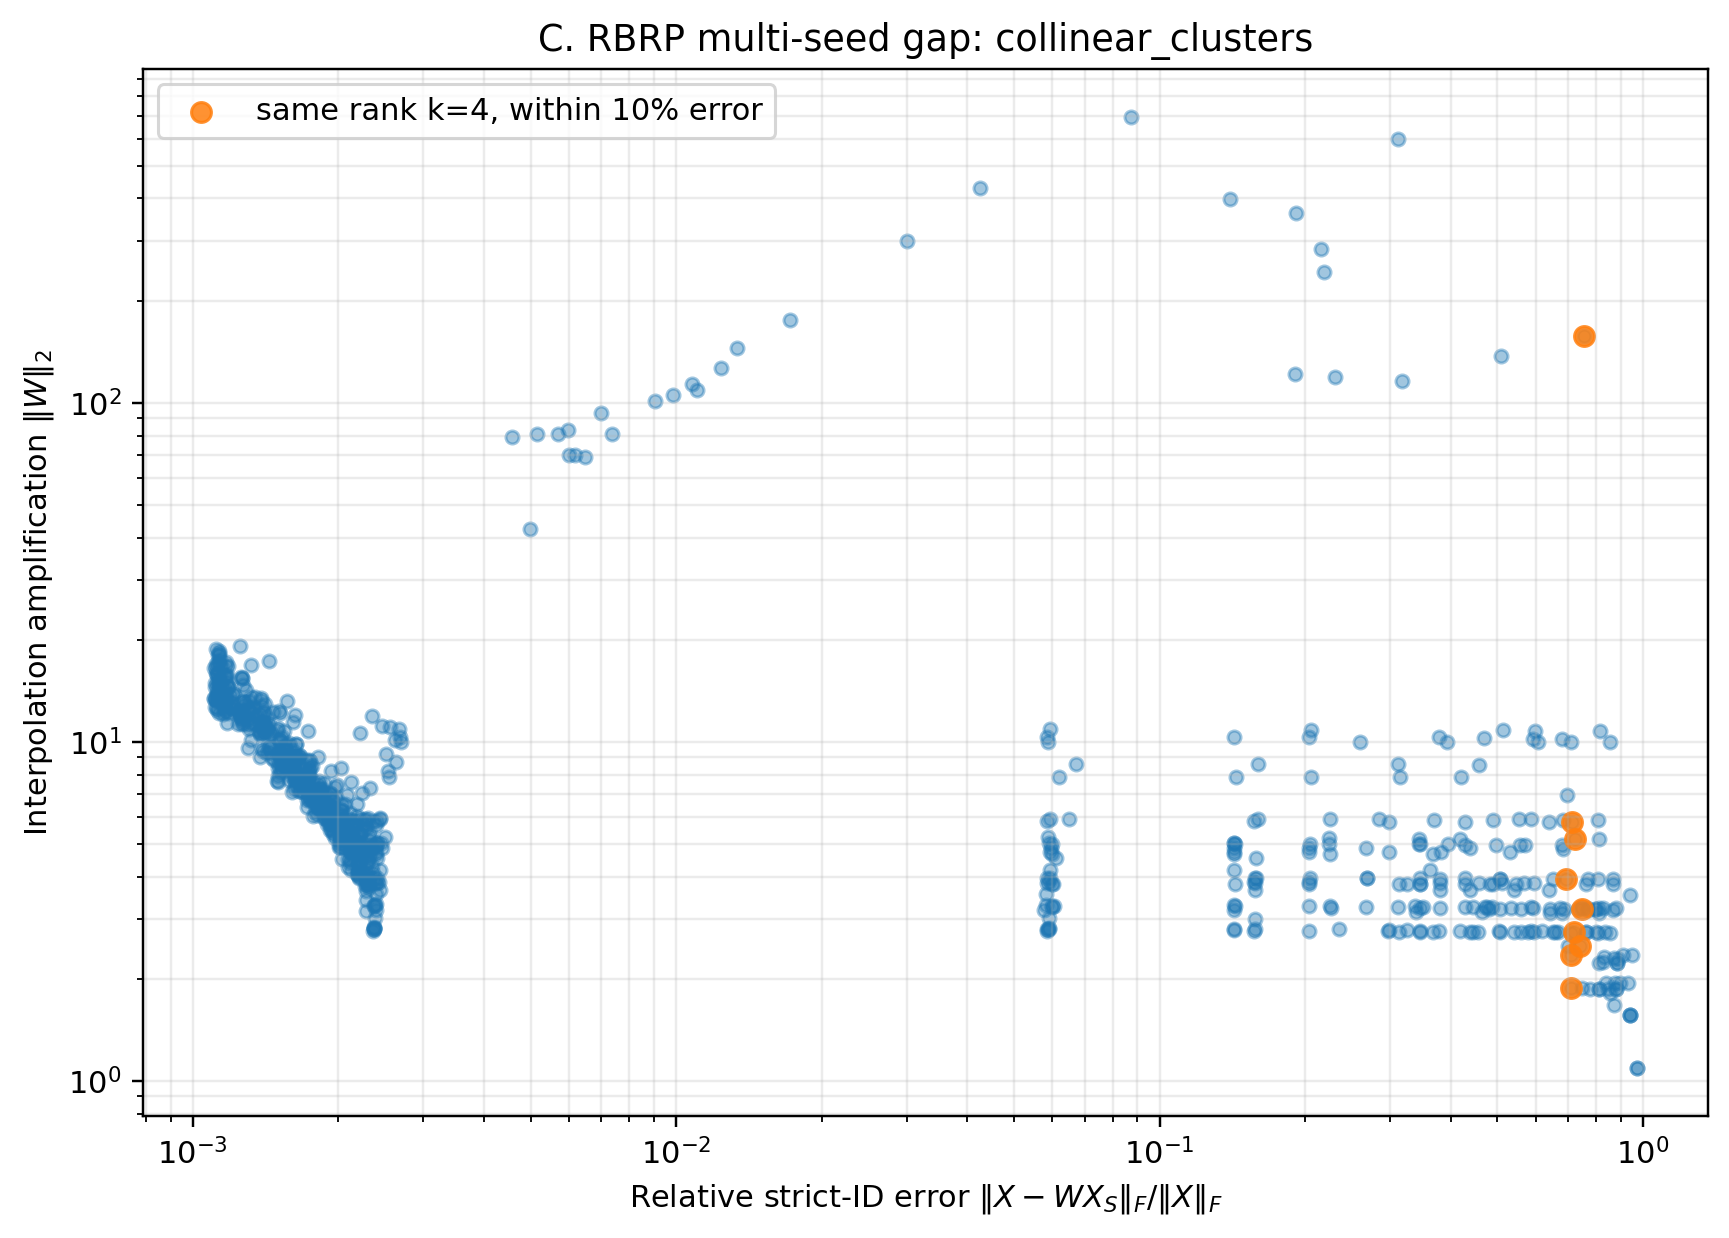
\includegraphics[width=\textwidth]{figs/s1_collinear_clusters.png}\end{subfigure}\hfill
\begin{subfigure}{.48\textwidth}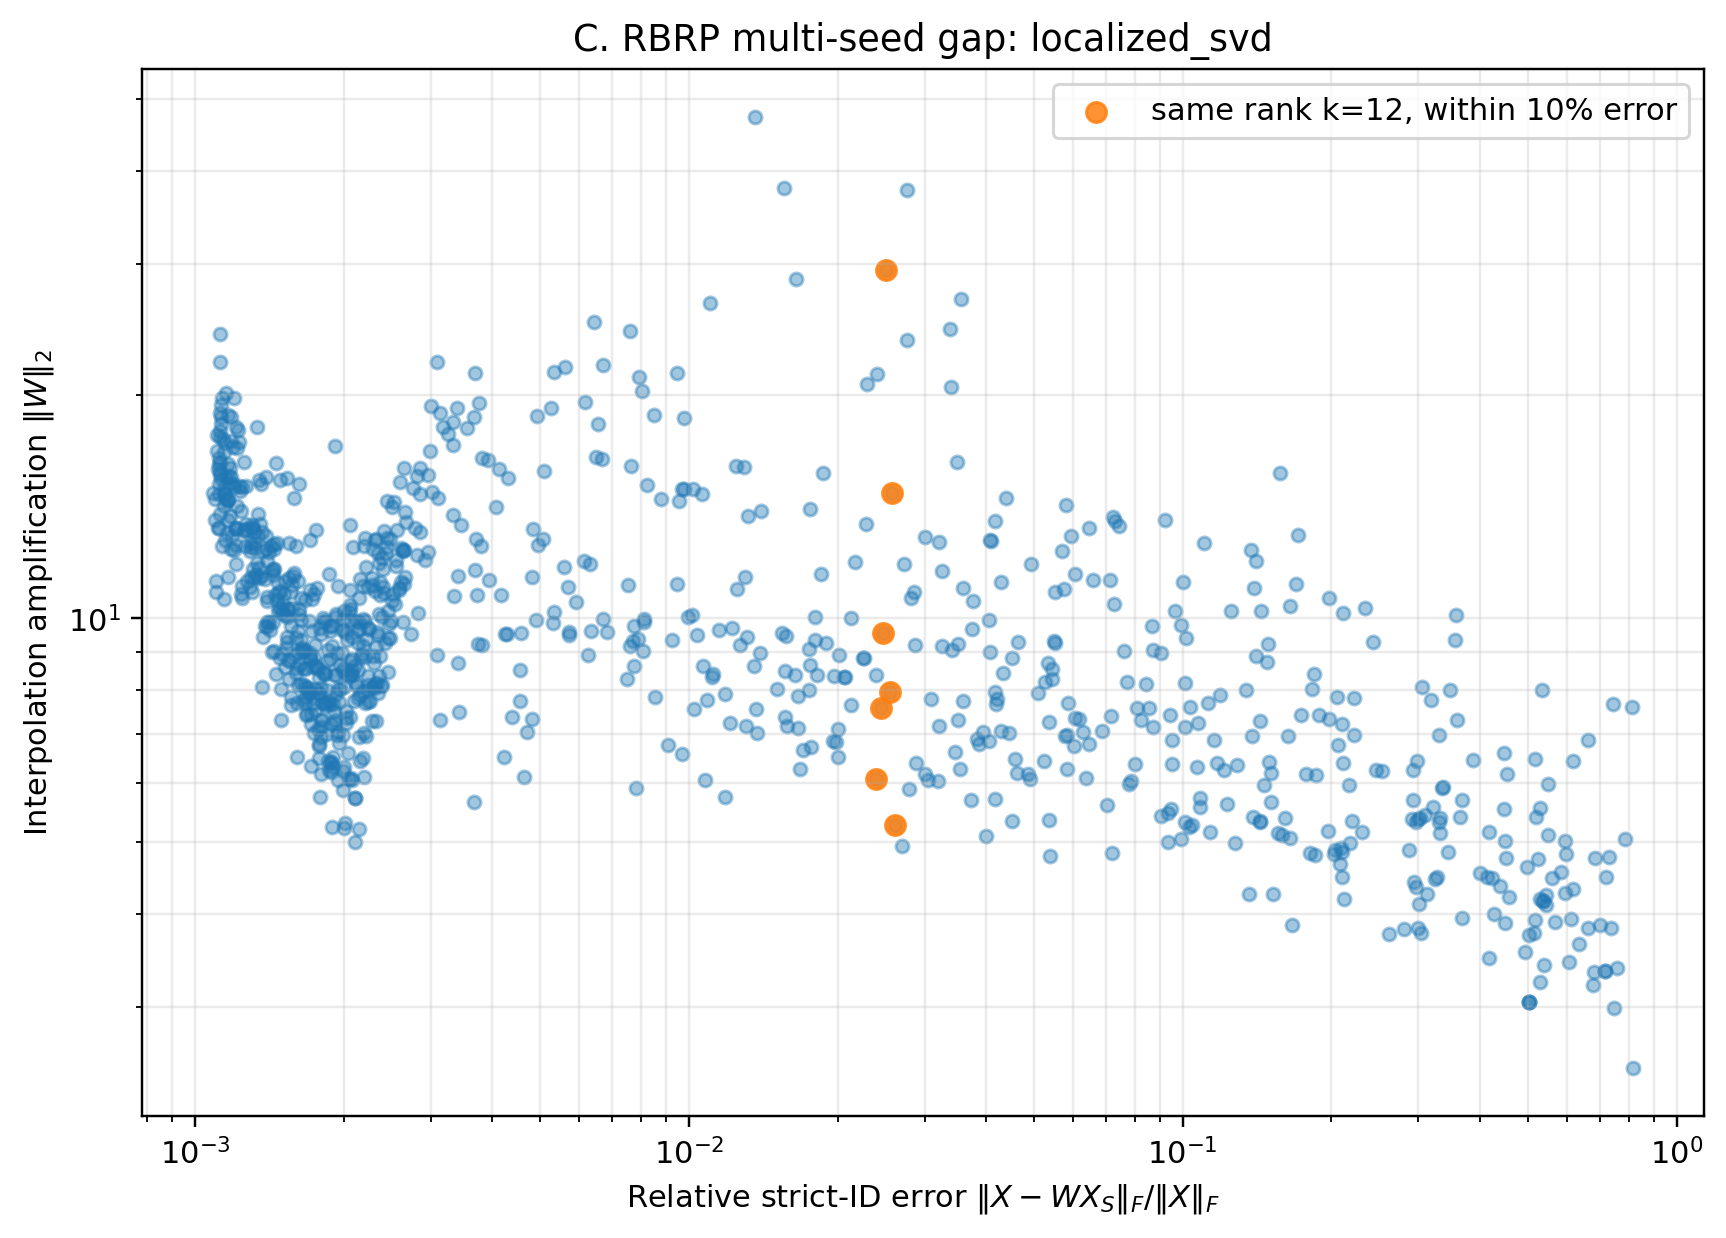
\includegraphics[width=\textwidth]{figs/s1_localized_svd.png}\end{subfigure}\\[2mm]
\begin{subfigure}{.48\textwidth}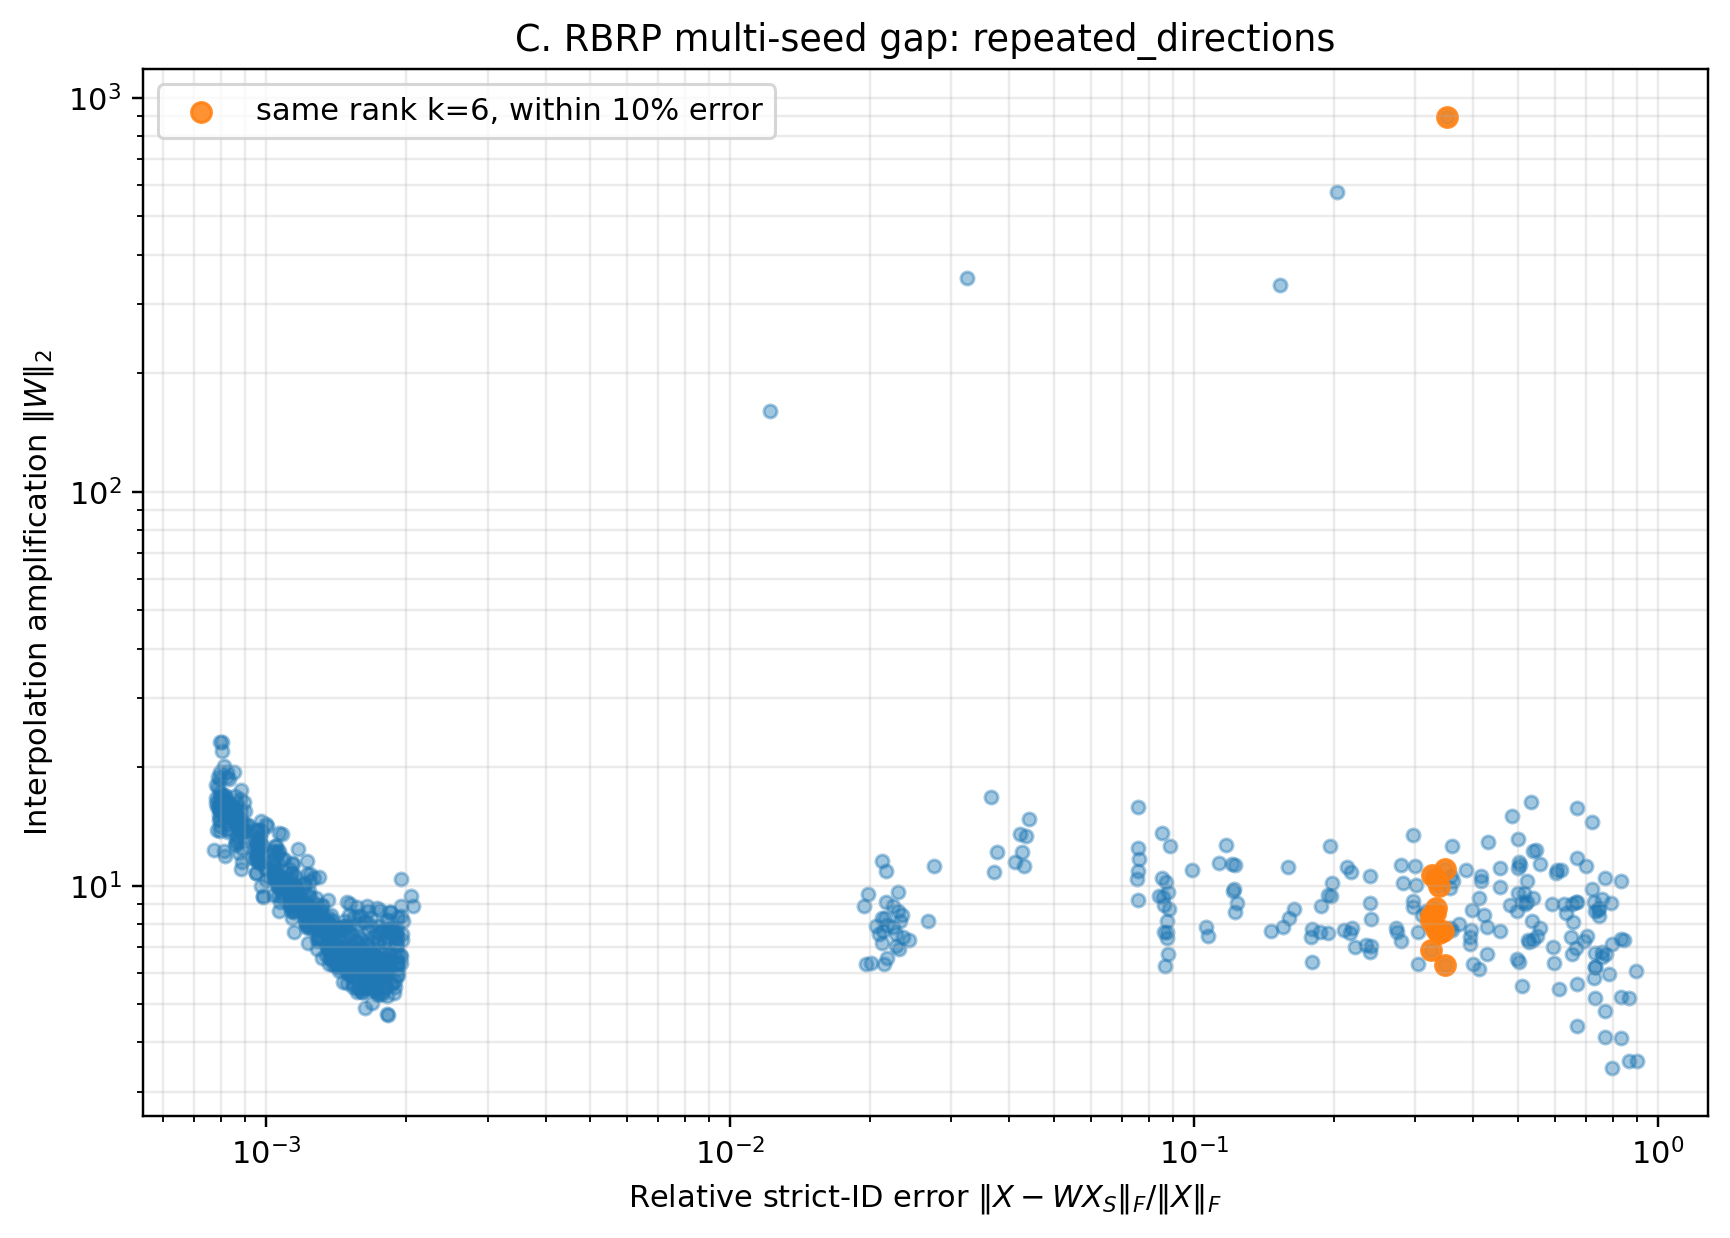
\includegraphics[width=\textwidth]{figs/s1_repeated_directions.png}\end{subfigure}\hfill
\begin{subfigure}{.48\textwidth}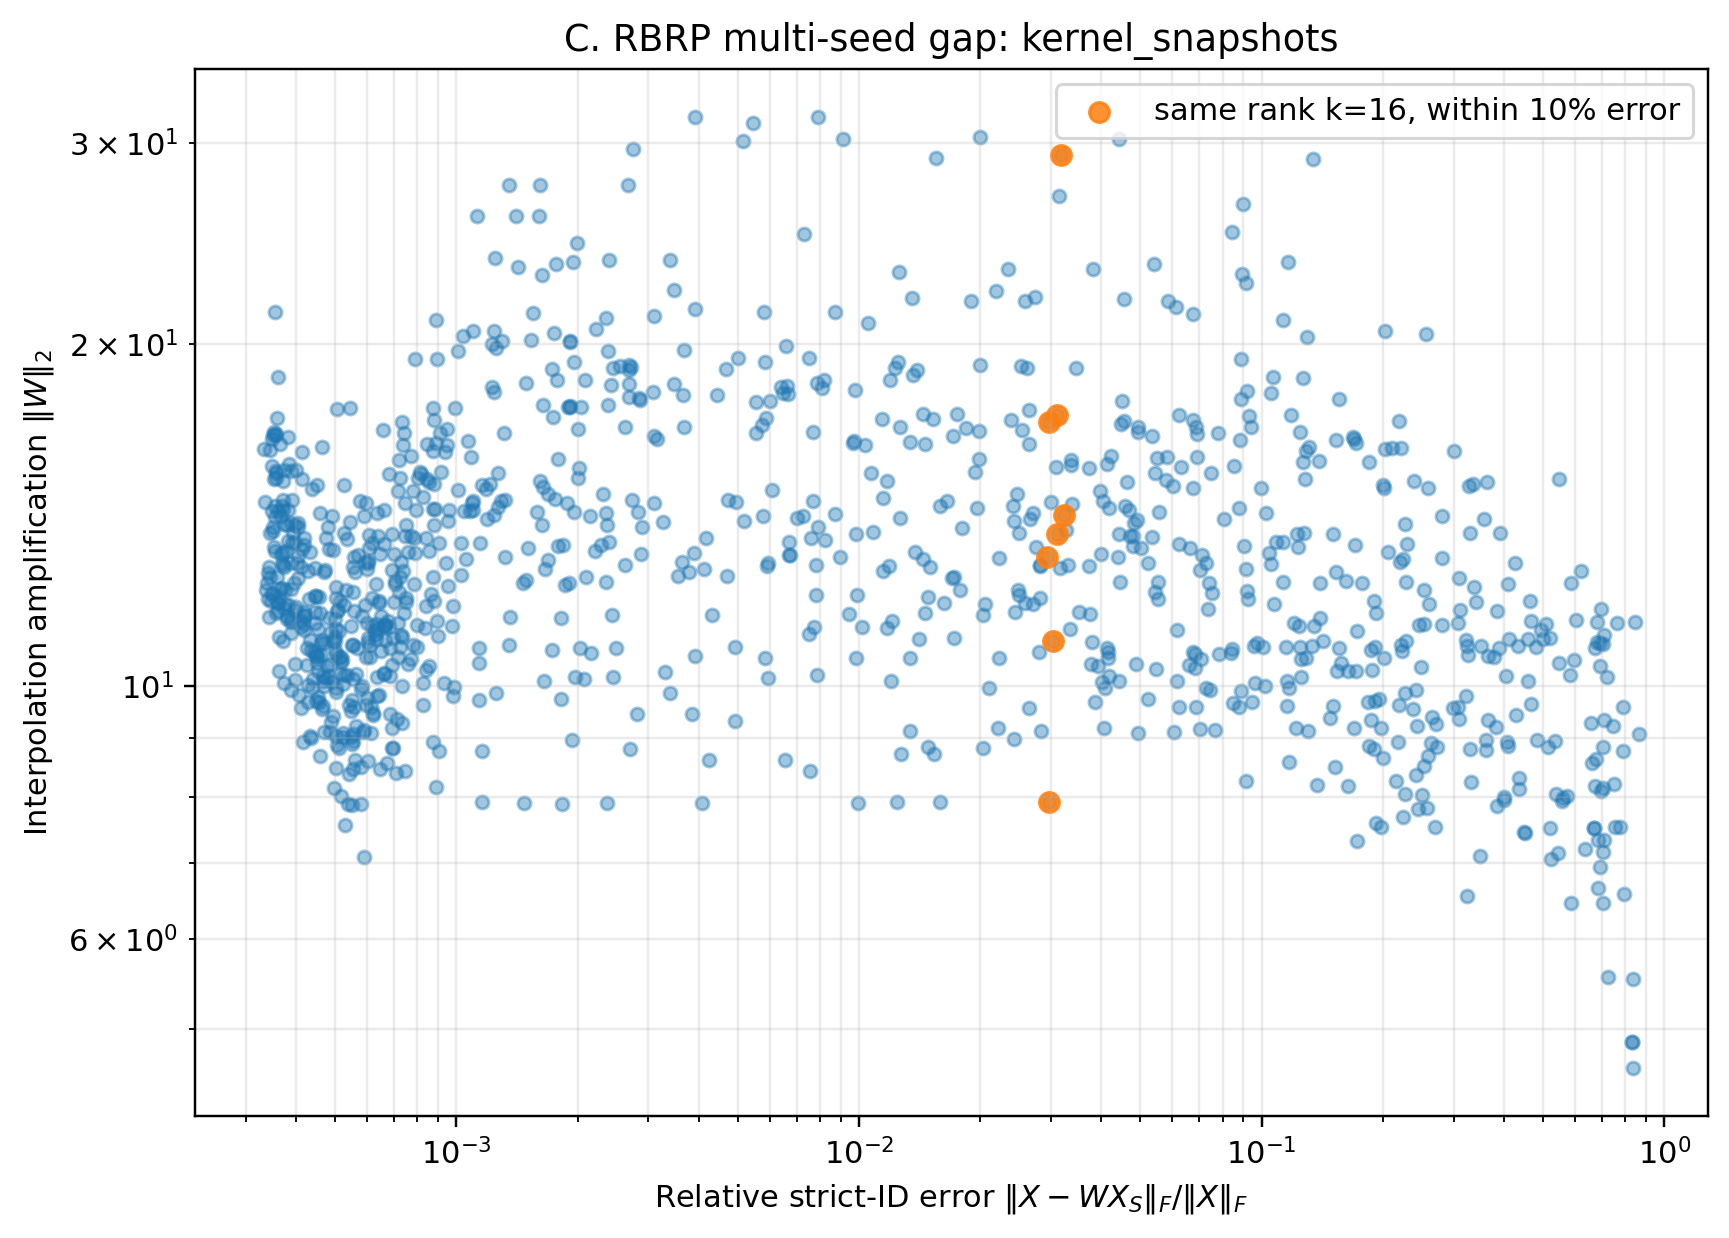
\includegraphics[width=\textwidth]{figs/s1_kernel_snapshots.png}\end{subfigure}
\caption{Error versus amplification of the RBRP skeletons of 40 seeds (all ranks); the orange points form the window of the largest matched gap.}\label{fig:stage1}
\end{figure}
Two caveats apply.
The gap is a \emph{largest} ratio over windows that contain only $5$--$14$ skeletons, so it shows what can happen for skeletons of equal size and similar error, not what is typical; the scatter plots in Figure~\ref{fig:stage1} show the typical spread.
And the diagnostic matrices are the synthetic families, not application matrices.
This supports only the claim that the approximation error does not by itself control the amplification of RBRP skeletons; it is not a theorem.

\subsection{Error-budgeted exchange refinement}
Algorithm~\ref{alg:ref} orders the non-skeleton rows by $\|W(i,:)\|_2$ because $A(S)\ge\max_i\|W(i,:)\|_2$ by \eqref{eq:A}: the row with the largest norm is a direct source of amplification.
The ordering only decides which row is tried first.

\begin{algorithm}[t]
\caption{Error-budgeted exchange refinement $\textsc{Refine}(X,S_0,\varepsilon,T)$}\label{alg:ref}
\begin{algorithmic}[1]
\State $E_0\gets E(S_0)$; $S\gets S_0$
\Repeat
  \State $W\gets XX_S^\dagger$; order $N=\{1,\dots,n\}\setminus S$ by decreasing $\|W(i,:)\|_2$ (stable ties); keep the first $T$ entries
  \For{$i$ in this order}
    \State $\mathcal C\gets\{S'=(S\setminus\{s_j\})\cup\{i\}:\ S'\text{ valid},\ E(S')\le(1+\varepsilon)E_0,\ A(S')<(1-\tau)A(S),\ j=1,\dots,k\}$
    \If{$\mathcal C\neq\emptyset$} $S\gets\arg\min_{S'\in\mathcal C}A(S')$ (ties: smaller $E$); \textbf{break} \EndIf
  \EndFor
\Until{no accepted exchange in the last pass}
\State \Return $S$
\end{algorithmic}
\end{algorithm}
Here $\tau=10^{-12}$ prevents floating-point cycling.
With $T=\infty$ the algorithm is parameter-free and deterministic; $T<\infty$ is the budgeted variant.

\subsection{Volume-based exchange and the two-stage pipeline}
Let $U\in\R^{n\times k}$ contain the top-$k$ left singular vectors of $X$ and $\hat A=UU_S^{-1}$.
Exchanging row $i$ for $s_j$ multiplies $|\det U_S|$ by $|\hat A_{ij}|$ and updates $\hat A$ by a rank-one formula \cite{goreinov2010}.
\emph{Vol$(f)$} repeatedly performs the exchange with the largest $|\hat A_{ij}|$ while it exceeds $f$ ($f=1$: locally maximal volume).
It uses only $U$ and does not look at $E$; afterwards we evaluate the exact $A$ and $E$ of the result.
\emph{VolGuard} performs the same exchanges in decreasing order of $|\hat A_{ij}|$ (at most $500$ candidates per iteration) but accepts one only if the exact error satisfies $E(S')\le(1+\varepsilon)E_0$.

\begin{algorithm}[t]
\caption{Two-stage pipeline $\textsc{Hybrid}(X,S_0,\varepsilon,T)$}\label{alg:hyb}
\begin{algorithmic}[1]
\State $S_1\gets$ VolGuard$(X,S_0,f{=}1,\varepsilon)$ \Comment{cheap, guarded by $E_0=E(S_0)$}
\State $S_f\gets\textsc{Refine}(X,S_1,\varepsilon,T)$ with the budget still relative to $E_0$
\State \Return $S_f$
\end{algorithmic}
\end{algorithm}

\section{Properties}\label{sec:analysis}
\begin{proposition}[Guarantees of Algorithm~\ref{alg:ref}]\label{prop:ref}
Let $S_0$ be valid. (a) Every iterate is valid and satisfies $E(S)\le(1+\varepsilon)E_0$. (b) $A$ decreases by at least a factor $(1-\tau)$ at each accepted exchange; hence the algorithm terminates after finitely many steps. (c) If $T=\infty$, the output $S_f$ is a single-exchange local optimum: no exchange $S'$ with $E(S')\le(1+\varepsilon)E_0$ has $A(S')<(1-\tau)A(S_f)$. (d) For $T<T'$ and the same tie-breaking, the trajectory with budget $T$ is a prefix of that with $T'$; hence $A(S_f^{(T')})\le A(S_f^{(T)})$.
\end{proposition}
\begin{proof}
(a), (b): by construction an exchange is accepted only if it is valid, satisfies the budget and decreases $A$; there are finitely many $k$-subsets, and $A$ cannot return to a previous value.
(c): the algorithm stops only after a pass in which every non-skeleton row has been tried without an accepted exchange.
(d): the two runs choose the same exchange as long as the budgeted run finds an admissible exchange among its first $T$ rows, because both pick the first row in the order that admits one and the best exchange for that row; when the budgeted run stops, the other run continues from the same skeleton and can only decrease $A$ further.
\end{proof}

\begin{proposition}[Exact-rank case]\label{prop:rank}
If $\operatorname{rank}X=k$ and $U\in\R^{n\times k}$ has orthonormal columns spanning the column space of $X$, then for every valid $S$, $E(S)=0$, $W=UU_S^{-1}$ and $A(S)=\|U_S^{-1}\|_2=1/\sigma_{\min}(U_S)$.
\end{proposition}
\begin{proof}
Write $X=UB$ with $B\in\R^{k\times d}$ of full row rank. Then $X_S=U_SB$ with $U_S$ invertible, $X_S^\dagger=B^\dagger U_S^{-1}$ and $W=UBB^\dagger U_S^{-1}=UU_S^{-1}$. Since $U$ has orthonormal columns, $\|W\|_2=\|U_S^{-1}\|_2$.
\end{proof}
Hence in the exact-rank case $A(S)$ coincides with the DEIM error constant $\|(P^TU)^{-1}\|_2$ \cite{chaturantabut2010,drmac2016}, and $\|W\|_2^{-1}=\sigma_{\min}(U_S)$, which is the quantity that volume maximization controls only indirectly through $\det U_S$.

\begin{proposition}[Pipeline]\label{prop:hyb}
Algorithm~\ref{alg:hyb} returns a valid skeleton with $E(S_f)\le(1+\varepsilon)E_0$ and $A(S_f)\le A(S_1)$.
\end{proposition}
This follows from Proposition~\ref{prop:ref}(a),(b), because the refinement is started from $S_1$ with the same budget. It says that the second stage cannot hurt; the size of the gain is an empirical question (Section~\ref{sec:exp}).

\begin{proposition}[Cost]\label{prop:cost}
One exact evaluation of $(A(S'),E(S'))$ costs $O(ndk)$ operations. A pass of Algorithm~\ref{alg:ref} with budget $T$ costs at most $Tk$ evaluations; with $T=\infty$ the last (certifying) pass costs $(n-k)k$ evaluations, i.e.\ $O(n^2dk^2)$ operations.
\end{proposition}

\begin{proposition}[Perturbed skeleton]\label{prop:pert}
Let $R=WX_S-X$ and let the skeleton rows be observed as $X_S+N$ with $N\in\R^{k\times d}$, $\hat X=W(X_S+N)$.
(a) If the entries of $N$ are i.i.d.\ $\mathcal N(0,\sigma^2)$, then $\mathbb E\|\hat X-X\|_F^2=\|R\|_F^2+\sigma^2d\|W\|_F^2$.
(b) For every $\delta>0$ there is $N$ with $\|N\|_F=\delta$ and $\|\hat X-X\|_F^2\ge\|R\|_F^2+\delta^2\|W\|_2^2$, and for all such $N$, $\|\hat X-X\|_F\le\|R\|_F+\delta\|W\|_2$.
\end{proposition}
\begin{proof}
(a) The cross term $2\langle R,WN\rangle$ has mean zero and $\mathbb E\|WN\|_F^2=\sigma^2d\|W\|_F^2$.
(b) Let $W=\sum_i\sigma_iu_iv_i^T$ and $N=\delta v_1w^T$ with $w\in\R^d$ a unit vector chosen so that $\langle R,u_1w^T\rangle\ge0$ (e.g.\ $w=\pm R^Tu_1/\|R^Tu_1\|$). Then $\|R+WN\|_F^2=\|R\|_F^2+2\delta\sigma_1\langle R,u_1w^T\rangle+\delta^2\sigma_1^2$. The upper bound is the triangle inequality.
\end{proof}
With $\sigma=\nu\|X\|_F/\sqrt{nd}$, (a) gives the relative error $\sqrt{E^2+\nu^2\|W\|_F^2/n}$.
Thus the amplification $\|W\|_2$ controls the worst case, whereas random noise is controlled by $\|W\|_F\in[\sqrt k,\sqrt k\|W\|_2]$.

\begin{remark}
We do not prove an accuracy guarantee for the refined skeleton. Local search can end in poor local optima in general (cf.\ the analysis of exchange algorithms for optimal designs in \cite{madan2019}), and Proposition~\ref{prop:ref}(c) only says that no single exchange within the budget helps.
\end{remark}

\section{Numerical experiments}\label{sec:exp}
\subsection{Setup}
\paragraph{Matrices.}
Four synthetic datasets with $n=500$, $d=60$ (nearly collinear clusters, repeated directions, localized SVD, kernel snapshots) at representative ranks $k=4,4,14,16$; a Burgers snapshot matrix ($1000\times256$: 25 initial phases $\times$ 8 viscosities $\times$ 5 times of the periodic viscous Burgers equation, pseudo-spectral with a first-order IMEX step; $k=8,16,24$); and the scikit-learn handwritten digits ($1797\times64$; $k=10,20,30$).
\paragraph{Protocol.}
All methods start from the same RBRP skeleton ($b=4$); $\varepsilon=0.05$; $A$ and $E$ are always evaluated exactly on the full matrix.
Seeds: 40 per synthetic dataset in Section~\ref{sec:main}, 20 per configuration elsewhere; full scans on Burgers and digits $k{=}10$ use 10 seeds.
QRCP denotes QR with column pivoting applied to $X^T$.
Intervals are 95\% percentile bootstrap intervals (5000 resamples of the seeds within each configuration, keeping the pairing of the methods); pooled statistics are recomputed for every resample. The intervals quantify the randomness of RBRP for the given matrices; they do not capture the variation across matrices, which is only represented by the 19 configurations used.
Timings are single-threaded wall-clock times on one machine.

\subsection{Main experiment}\label{sec:main}
\begin{table}[t]
\centering\small
\caption{Main experiment on the four synthetic datasets ($n=500$, $d=60$, 40 RBRP seeds each). $\rho_A=A_f/A_0$ and $\rho_E=E_f/E_0$ are averaged over seeds.}\label{tab:pilot}
\begin{adjustbox}{max width=\linewidth}
\begin{tabular}{lrrrrrrr}
\toprule
Dataset & full $\rho_A$ & $T{=}10$ $\rho_A$ & full $\rho_E$ & evals (full) & evals ($T{=}10$) & time (s) full & time (s) $T{=}10$ \\
\midrule
Collinear clusters ($k=4$) & 0.522 & 0.573 & 1.007 & 3,215 & 51 & 2.4 & 0.04 \\
Repeated directions ($k=4$) & 0.433 & 0.464 & 0.994 & 2,291 & 71 & 1.8 & 0.06 \\
Localized SVD ($k=14$) & 0.380 & 0.392 & 0.793 & 7,119 & 296 & 7.8 & 0.32 \\
Kernel snapshots ($k=16$) & 0.356 & 0.419 & 0.942 & 15,222 & 658 & 17.2 & 0.76 \\
All (160 runs) & 0.423 & 0.462 & 0.934 & 6,962 & 269 & 7.3 & 0.29 \\
\bottomrule
\end{tabular}
\end{adjustbox}
\end{table}

Table~\ref{tab:pilot} shows that the full scan lowers the mean amplification to $42\%$ of the RBRP value with the error budget satisfied in all runs, and that the budgeted variant ($T=10$) obtains most of this at a small fraction of the evaluations.
In all 160 runs the full scan ended at a single-exchange local optimum, and an independent brute-force check of all $k(n-k)$ exchanges on 8 runs found no admissible exchange.

\subsection{Scan budget and ordering}
\begin{table}[t]
\centering\small
\caption{Scan budget $T$ and ordering ablation (160 runs, same $S_0$ for both orders).}\label{tab:tsweep}
\begin{adjustbox}{max width=\linewidth}
\begin{tabular}{lrrrr}
\toprule
$T$ & row-norm order $\rho_A$ (SE) & evals & random order $\rho_A$ (SE) & evals \\
\midrule
1 & 0.575 (0.020) & 33 & 0.948 (0.011) & 13 \\
2 & 0.535 (0.019) & 57 & 0.923 (0.012) & 30 \\
5 & 0.483 (0.017) & 143 & 0.857 (0.015) & 88 \\
10 & 0.462 (0.017) & 269 & 0.809 (0.016) & 257 \\
20 & 0.448 (0.017) & 591 & 0.728 (0.017) & 581 \\
50 & 0.438 (0.017) & 1,278 & 0.618 (0.018) & 1,818 \\
$\infty$ & 0.423 (0.016) & 6,962 & -- & -- \\
\bottomrule
\end{tabular}
\end{adjustbox}
\end{table}

\begin{figure}[t]\centering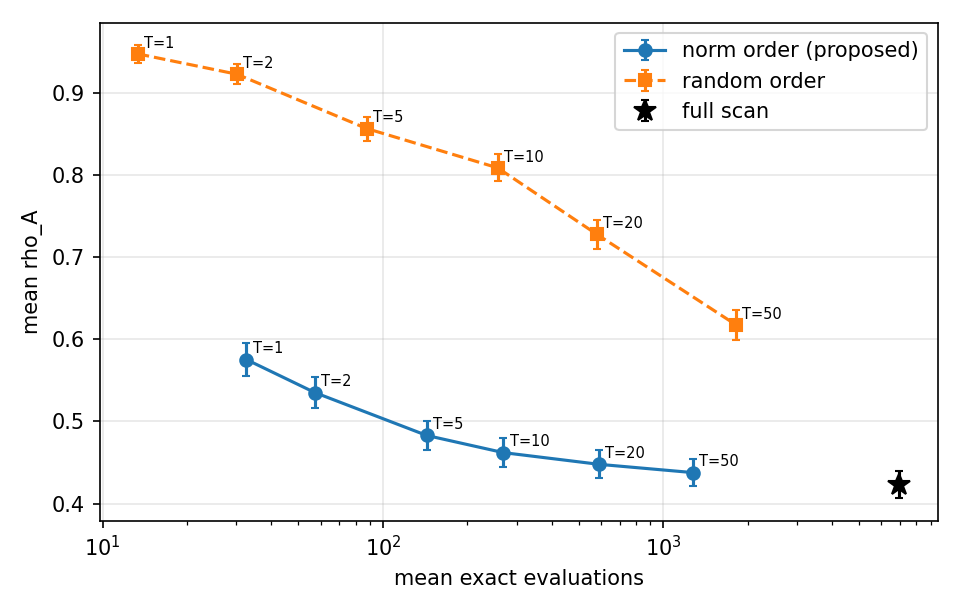
\includegraphics[width=.6\textwidth]{figs/tsweep.png}
\caption{Cost--benefit of the scan budget $T$: mean $\rho_A$ versus mean number of exact evaluations, for the row-norm order and for a random order.}\label{fig:tsweep}\end{figure}
Table~\ref{tab:tsweep} and Figure~\ref{fig:tsweep}: $\rho_A$ decreases monotonically with $T$ (by Proposition~\ref{prop:ref}(d) this holds run by run), with strongly diminishing returns.
At matched cost, ordering by $\|W(i,:)\|_2$ is far better than a random order (for $T=10$: $0.462$ versus $0.809$ with $269$ versus $257$ evaluations); the row-norm order was better in $89$--$96\%$ of the paired runs.
$T=10$ retains about $93\%$ of the full-scan reduction at $4\%$ of its evaluations; this value was chosen from the same sweep and is a representative operating point, not a tuned constant.

\subsection{Rank sensitivity}
\begin{table}[t]
\centering\small
\caption{Rank sensitivity (20 seeds per configuration).}\label{tab:rank}
\begin{adjustbox}{max width=\linewidth}
\begin{tabular}{lrrrr}
\toprule
Dataset & $k$ & median $A_0$ & full $\rho_A$ (SE) & $T{=}10$ $\rho_A$ (SE) \\
\midrule
Kernel snapshots & 8 & 12.3 & 0.475 (0.033) & 0.509 (0.038) \\
Kernel snapshots & 12 & 14.4 & 0.401 (0.029) & 0.447 (0.041) \\
Kernel snapshots & 16 & 15.1 & 0.348 (0.033) & 0.401 (0.042) \\
Kernel snapshots & 20 & 15.4 & 0.391 (0.031) & 0.440 (0.036) \\
Localized SVD & 6 & 15.9 & 0.333 (0.042) & 0.347 (0.045) \\
Localized SVD & 10 & 17.0 & 0.347 (0.047) & 0.355 (0.046) \\
Localized SVD & 14 & 17.3 & 0.313 (0.037) & 0.325 (0.039) \\
Localized SVD & 18 & 15.6 & 0.374 (0.038) & 0.393 (0.041) \\
Collinear clusters & 4 & 5.1 & 0.498 (0.048) & 0.556 (0.057) \\
Collinear clusters & 6 & 4.4 & 0.520 (0.049) & 0.556 (0.052) \\
Collinear clusters & 8 & 5.6 & 0.474 (0.038) & 0.485 (0.038) \\
Collinear clusters & 12 & 5.1 & 0.576 (0.051) & 0.576 (0.051) \\
Repeated directions & 4 & 9.8 & 0.446 (0.021) & 0.474 (0.020) \\
Repeated directions & 6 & 11.4 & 0.433 (0.032) & 0.450 (0.033) \\
Repeated directions & 8 & 10.7 & 0.490 (0.026) & 0.490 (0.026) \\
Repeated directions & 10 & 7.3 & 0.530 (0.037) & 0.530 (0.037) \\
\bottomrule
\end{tabular}
\end{adjustbox}
\end{table}

\begin{figure}[t]\centering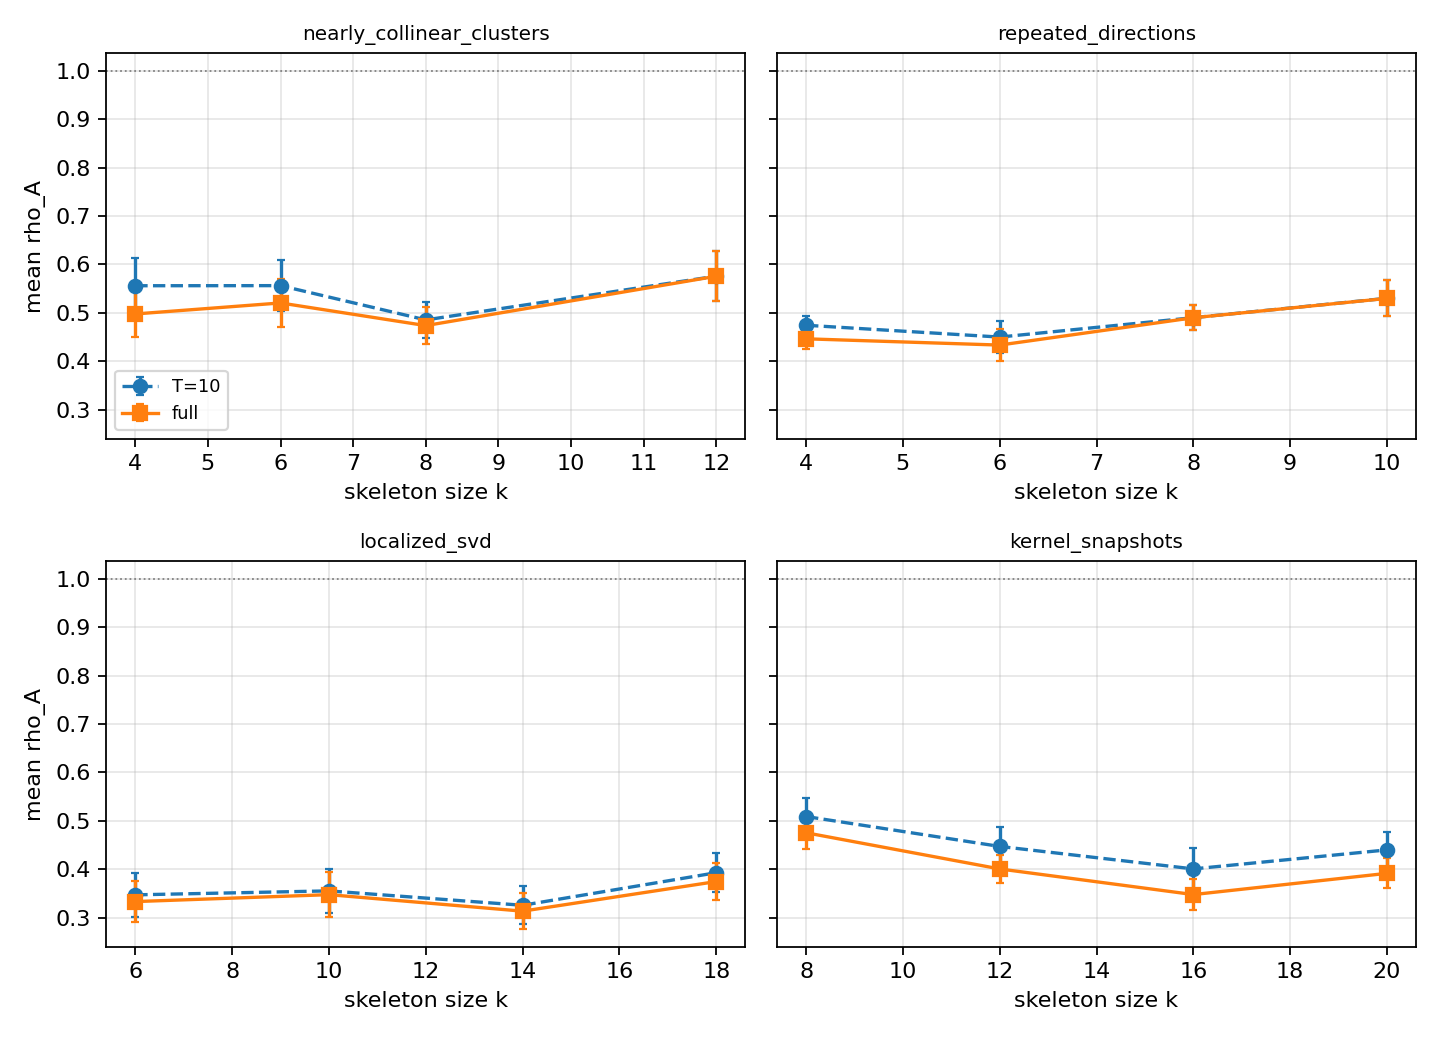
\includegraphics[width=.8\textwidth]{figs/rank.png}
\caption{Mean $\rho_A$ versus the skeleton size $k$ ($T=10$ and full scan).}\label{fig:rank}\end{figure}
Table~\ref{tab:rank} and Figure~\ref{fig:rank}: the reduction is present at every tested rank (mean $\rho_A<1$ in all 16 configurations); there is no systematic trend with $k$, and differences between neighbouring ranks are mostly within one or two standard errors.

\subsection{Comparison with volume-based exchange and the pipeline}
\begin{table}[t]
\centering\small
\caption{Median amplification $A$ after each method (20 RBRP seeds; the full scan uses 10 seeds on Burgers and digits $k{=}10$ and none on digits $k{=}20,30$). The last column is the share of Vol(1) runs satisfying $E\le1.05E_0$.}\label{tab:compare}
\begin{adjustbox}{max width=\linewidth}
\begin{tabular}{lrrrrrrrr}
\toprule
Matrix & $k$ & RBRP & Vol(1) & VolGuard & Ours-$T$10 & Hybrid & Ours-full & Vol(1) feasible \\
\midrule
Burgers & 8 & 17.7 & 13.2 & 13.1 & 13.1 & 12.4 & 9.3 & 0\% \\
Burgers & 16 & 21.4 & 8.0 & 12.8 & 13.6 & 11.1 & 8.1 & 0\% \\
Burgers & 24 & 26.9 & 11.6 & 12.3 & 12.6 & 12.2 & 10.8 & 35\% \\
Digits & 10 & 17.6 & 15.2 & 15.2 & 14.8 & 14.0 & 12.5 & 100\% \\
Digits & 20 & 18.9 & 15.7 & 15.7 & 15.1 & 14.0 & -- & 100\% \\
Digits & 30 & 24.3 & 16.0 & 16.0 & 16.8 & 14.4 & -- & 100\% \\
Kernel snapshots & 16 & 15.1 & 6.4 & 6.1 & 6.3 & 5.9 & 5.6 & 55\% \\
Localized SVD & 14 & 17.3 & 4.8 & 4.8 & 4.7 & 4.4 & 4.5 & 95\% \\
Collinear clusters & 4 & 5.1 & 2.6 & 2.6 & 2.4 & 2.6 & 2.2 & 100\% \\
Repeated directions & 4 & 9.8 & 4.5 & 4.5 & 4.5 & 4.3 & 4.2 & 95\% \\
\bottomrule
\end{tabular}
\end{adjustbox}
\end{table}

\begin{table}[t]
\centering\small
\caption{Paired comparison pooled over all configurations and seeds, with 95\% percentile bootstrap intervals (seeds resampled within configuration). ``x dominates y'' means no worse in both $A$ and $E$ and strictly better in one.}\label{tab:pooled}
\begin{adjustbox}{max width=\linewidth}
\begin{tabular}{llrrrrr}
\toprule
x & y & pairs & median $A$ ratio & median $E$ ratio & x dominates (\%) & y dominates (\%) \\
\midrule
Ours-T10 & Vol(f=1) & 200 & 0.998 [0.992, 1.013] & 1.055 [1.041, 1.070] & 13.0 [9.0, 17.0] & 23.0 [18.0, 28.0] \\
Ours-T10 & VolGuard-500 & 200 & 0.997 [0.985, 1.004] & 1.067 [1.050, 1.078] & 7.5 [4.0, 11.0] & 30.0 [24.0, 36.0] \\
Hybrid-T10 & VolGuard-500 & 200 & 0.963 [0.937, 0.976] & 1.001 [1.000, 1.007] & 18.0 [13.5, 23.0] & 0.0 [0.0, 0.0] \\
Hybrid-T10 & Ours-T10 & 200 & 0.946 [0.927, 0.967] & 0.983 [0.970, 0.990] & 40.5 [34.5, 46.5] & 5.5 [2.5, 9.0] \\
Hybrid-T10 & Vol(f=1) & 200 & 0.973 [0.952, 0.984] & 1.000 [1.000, 1.000] & 25.0 [20.0, 30.0] & 0.0 [0.0, 0.0] \\
Ours-T10-noG & Vol(f=1) & 200 & 0.936 [0.920, 0.953] & 1.095 [1.086, 1.112] & 16.5 [13.0, 20.0] & 24.0 [18.5, 29.5] \\
Ours-full & VolGuard-500 & 120 & 0.874 [0.843, 0.896] & 1.060 [1.043, 1.088] & 22.5 [17.5, 28.3] & 7.5 [3.3, 12.5] \\
Ours-full & Hybrid-T10 & 120 & 0.921 [0.894, 0.945] & 1.021 [1.008, 1.034] & 25.0 [19.2, 30.8] & 11.7 [6.7, 16.7] \\
Ours-full & Vol(f=1) & 120 & 0.903 [0.882, 0.926] & 1.054 [1.024, 1.085] & 30.8 [25.0, 37.5] & 6.7 [3.3, 10.8] \\
\bottomrule
\end{tabular}
\end{adjustbox}
\end{table}

\begin{figure}[t]\centering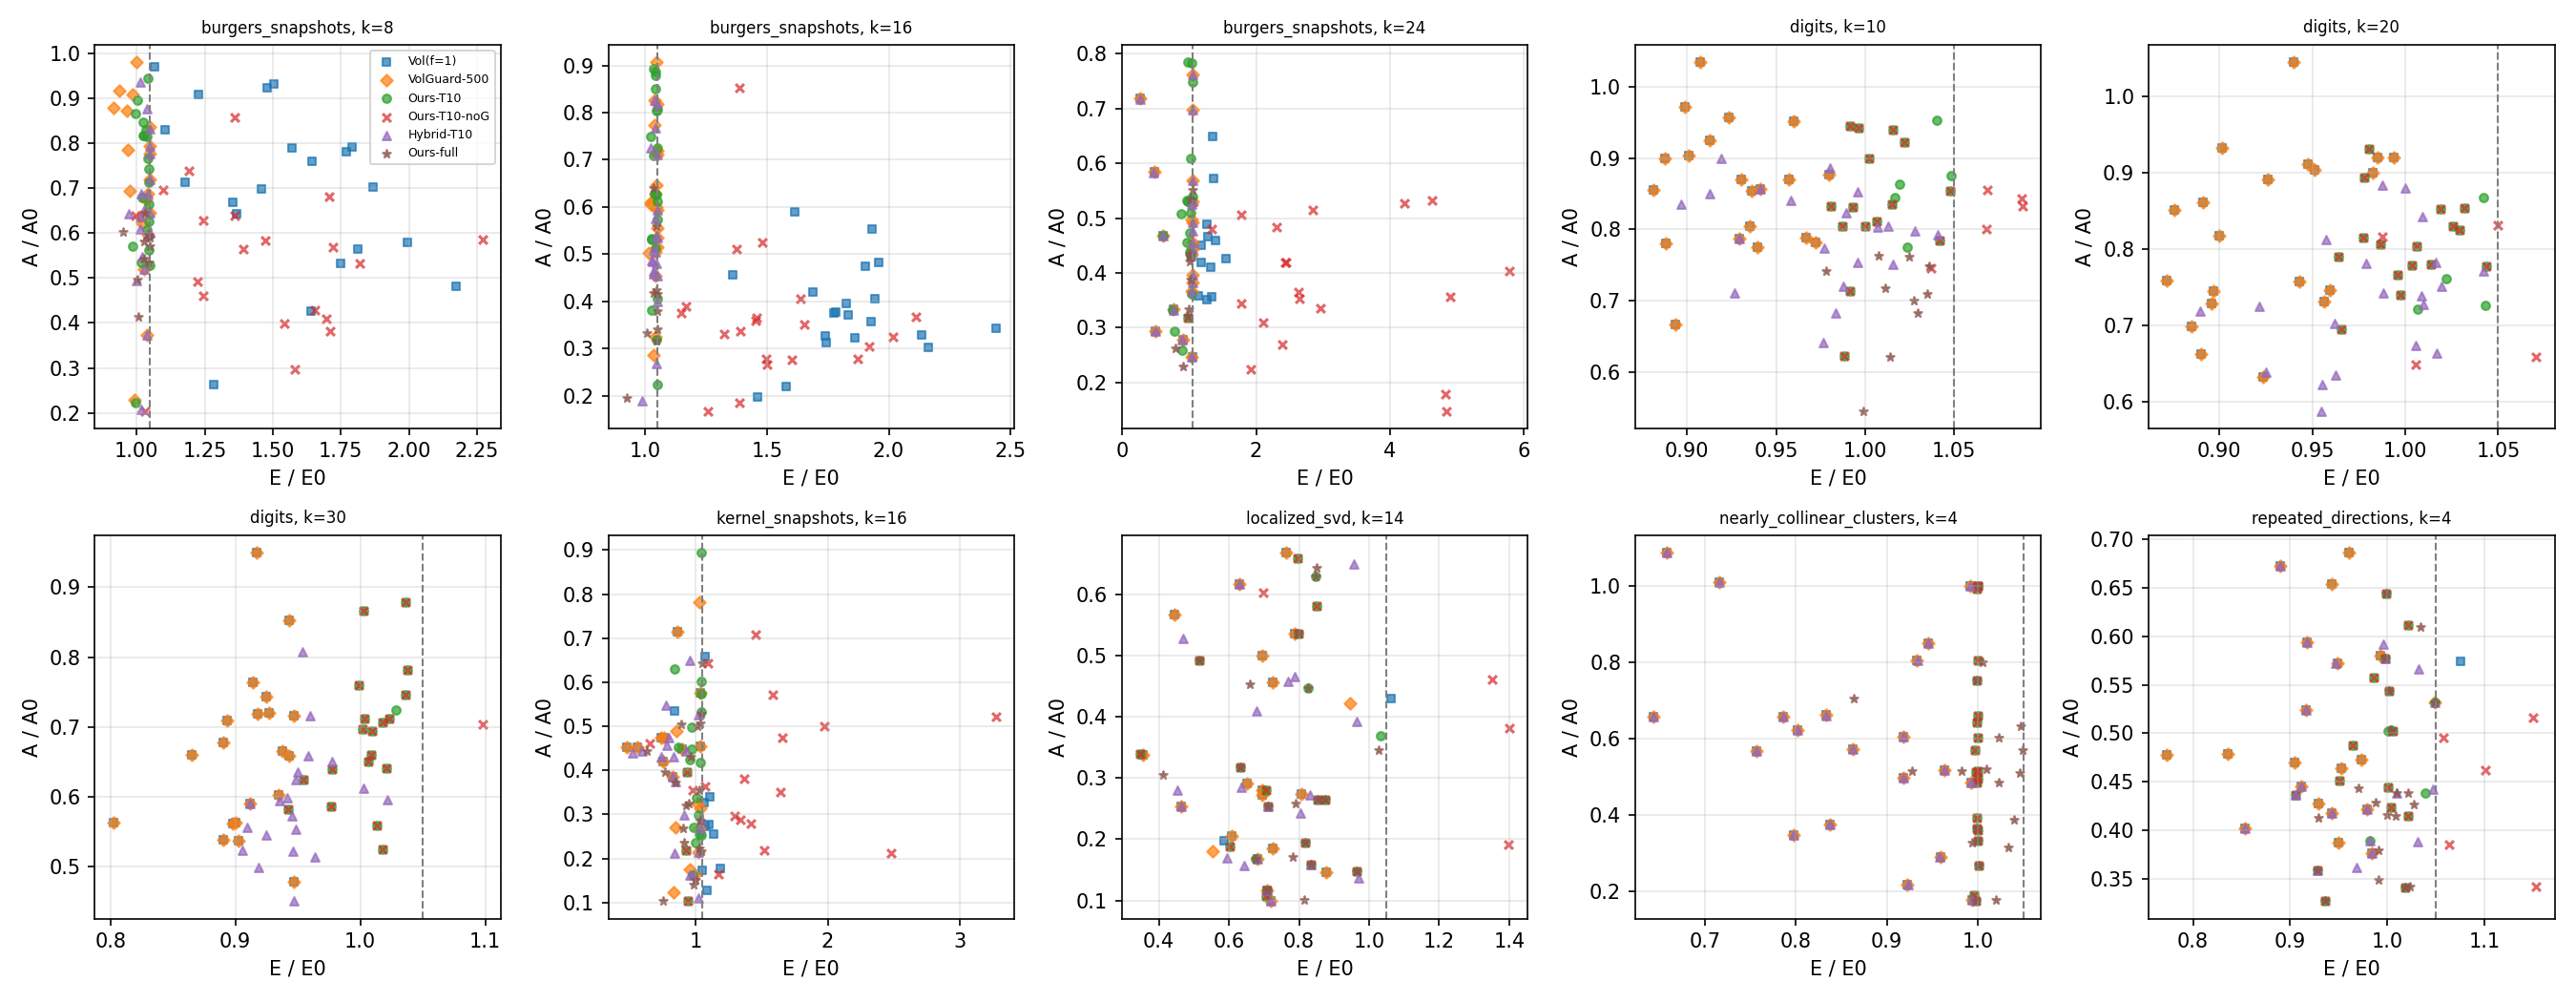
\includegraphics[width=\textwidth]{figs/scatter.png}
\caption{Per-run $(E/E_0,A/A_0)$ for the compared methods; the dashed line is the budget $1.05$.}\label{fig:scatter}\end{figure}
Tables~\ref{tab:compare} and \ref{tab:pooled} and Figure~\ref{fig:scatter} give the main comparison.
\begin{itemize}
\item Every post-processing method lowers the median amplification of the RBRP skeleton; the median over all runs of $A(\text{RBRP})/A(\text{pipeline})$ is $1.78$ (95\% interval $1.70$--$1.90$).
\item Unguarded volume exchange violates the budget in 64 of 200 runs ($32\%$, 95\% Wilson interval $26$--$39\%$; maximum $E=2.44E_0$; all runs on Burgers $k=8,16$); the guarded methods satisfy it in all runs.
\item At $T=10$ the refinement alone is not better than guarded volume exchange: the median $A$ ratio is $0.997$ ($0.985$--$1.004$, no detectable difference) and the median error ratio is $1.067$ ($1.050$--$1.078$); the guarded volume exchange dominates in $30\%$ ($24$--$36\%$) of the pairs, the refinement in $7.5\%$ ($4$--$11\%$).
\item The pipeline improves on the guarded volume exchange: median $A$ ratio $0.963$ ($0.937$--$0.976$) at an unchanged error (ratio $1.001$, $1.000$--$1.007$); it dominates in $18\%$ ($13.5$--$23\%$) of the pairs and, by construction, is never dominated. Against the refinement alone the median $A$ ratio is $0.946$ ($0.927$--$0.967$); the pipeline dominates in $40.5\%$ ($34.5$--$46.5\%$) of the pairs and is dominated in $5.5\%$ ($2.5$--$9\%$). The gain is concentrated: it is largest on Burgers $k=16$ (median ratio $0.857$; interval $0.81$--$0.995$) and about $8$--$10\%$ on digits, while the pipeline coincides with the guarded volume exchange in $40$--$60\%$ of the runs on Burgers $k=24$, collinear clusters and repeated directions. The order matters: on collinear clusters the refinement started from the RBRP skeleton is better than the pipeline, because the volume stage ends in a local volume maximum from which the refinement finds nothing.
\item A full scan is clearly better under the same budget: median $A$ ratio $0.874$ ($0.843$--$0.896$) against the guarded volume exchange and $0.921$ ($0.894$--$0.945$) against the pipeline, at roughly $30$--$240$ times the cost of the pipeline.
\end{itemize}
As the sign of the difference between the pipeline (or the full scan) and the method it starts from is determined by construction, we report intervals for the size of the gain rather than significance tests.

\subsection{Error budget}
\begin{table}[t]
\centering\small
\caption{Error-budget ablation (RBRP skeletons, $T{=}10$, 10 seeds). Each cell: median $A$ / mean $\rho_E$.}\label{tab:guard}
\begin{adjustbox}{max width=\linewidth}
\begin{tabular}{lrrrrr}
\toprule
Matrix & $k$ & $g{=}1.00$ & $g{=}1.05$ & $g{=}1.20$ & $g{=}\infty$ \\
\midrule
Burgers & 8 & 13.40 / 0.981 & 12.69 / 1.030 & 10.96 / 1.166 & 10.06 / 1.526 \\
Burgers & 16 & 14.70 / 0.982 & 13.15 / 1.039 & 9.71 / 1.181 & 6.91 / 1.514 \\
Burgers & 24 & 13.11 / 0.943 & 13.11 / 0.975 & 12.17 / 1.045 & 9.87 / 3.264 \\
Digits & 10 & 14.83 / 0.988 & 15.00 / 1.011 & 14.64 / 1.023 & 14.64 / 1.023 \\
Digits & 20 & 15.38 / 0.982 & 15.66 / 1.017 & 15.39 / 1.007 & 15.39 / 1.007 \\
Digits & 30 & 17.49 / 0.984 & 16.51 / 1.001 & 16.43 / 1.008 & 16.43 / 1.008 \\
\bottomrule
\end{tabular}
\end{adjustbox}
\end{table}

\begin{figure}[t]\centering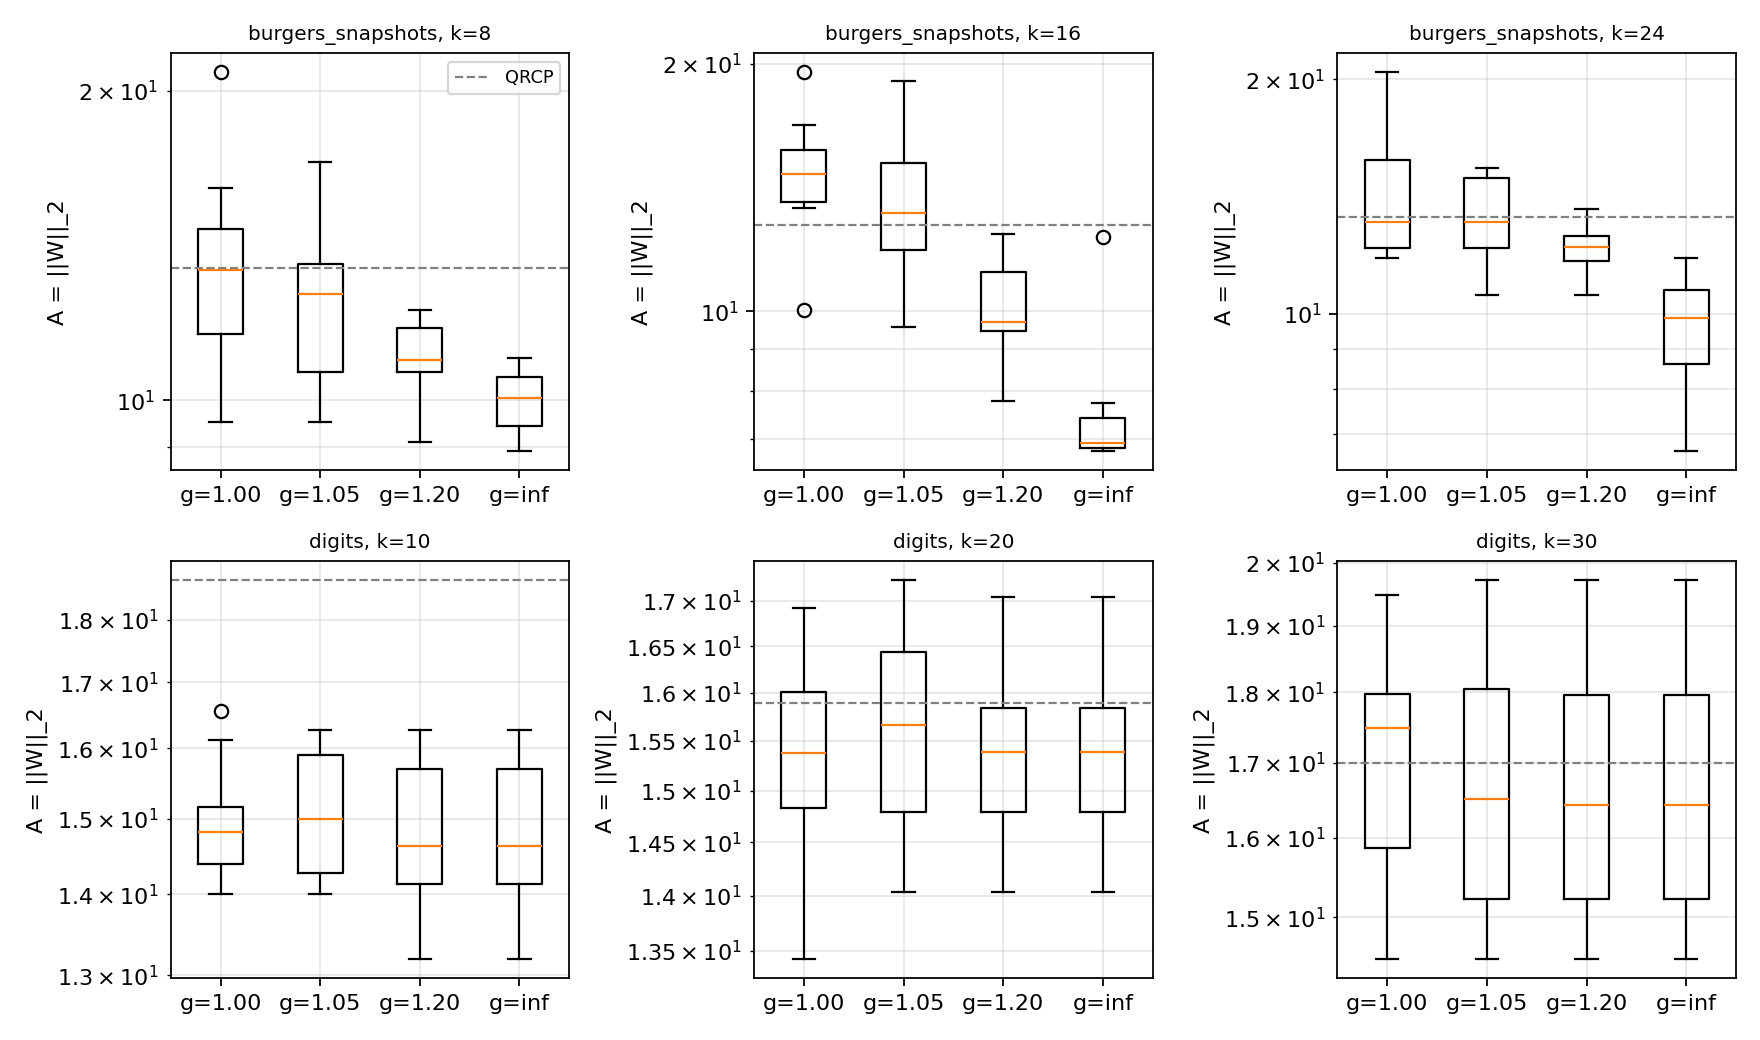
\includegraphics[width=\textwidth]{figs/guardA.png}
\caption{Amplification for different budgets $g$ (dashed: QRCP).}\label{fig:guard}\end{figure}
Table~\ref{tab:guard} and Figure~\ref{fig:guard}: on the Burgers matrix the budget is a genuine trade-off: removing it lowers the median amplification by a further $24$--$45\%$ but raises the median error by $39$--$159\%$ (up to $5.8E_0$); a moderate budget $g=1.20$ already gives much of the gain. On digits (with $T=10$) the budget has almost no effect. $\varepsilon=0.05$ is a working point, not an optimum.

\subsection{Cost and scaling}
\begin{table}[t]
\centering\small
\caption{Wall-clock time (single thread, $d=60$, representative $k$).}\label{tab:runtime}
\begin{adjustbox}{max width=\linewidth}
\begin{tabular}{lrrrrr}
\toprule
Dataset & $n$ & RBRP (ms) & $T{=}10$ (s) & $T{=}10$/RBRP & full (s) \\
\midrule
Kernel snapshots & 500 & 2.1 & 0.28 & 133 & 6.4 \\
Kernel snapshots & 1000 & 2.9 & 0.54 & 184 & 18.9 \\
Kernel snapshots & 2000 & 4.7 & 1.33 & 281 & 81.0 \\
Kernel snapshots & 4000 & 11.3 & 1.81 & 160 & -- \\
Localized SVD & 500 & 1.8 & 0.11 & 61 & 2.4 \\
Localized SVD & 1000 & 2.5 & 0.18 & 75 & 7.6 \\
Localized SVD & 2000 & 4.2 & 0.51 & 123 & 41.2 \\
Localized SVD & 4000 & 10.9 & 1.10 & 101 & -- \\
Collinear clusters & 500 & 0.8 & 0.01 & 17 & 0.6 \\
Collinear clusters & 1000 & 0.7 & 0.02 & 34 & 1.8 \\
Collinear clusters & 2000 & 1.4 & 0.05 & 35 & 8.9 \\
Collinear clusters & 4000 & 3.3 & 0.11 & 35 & -- \\
Repeated directions & 500 & 0.6 & 0.02 & 31 & 0.5 \\
Repeated directions & 1000 & 0.7 & 0.02 & 31 & 1.3 \\
Repeated directions & 2000 & 1.0 & 0.05 & 50 & 6.4 \\
Repeated directions & 4000 & 3.0 & 0.14 & 48 & -- \\
\bottomrule
\end{tabular}
\end{adjustbox}
\end{table}

\begin{figure}[t]\centering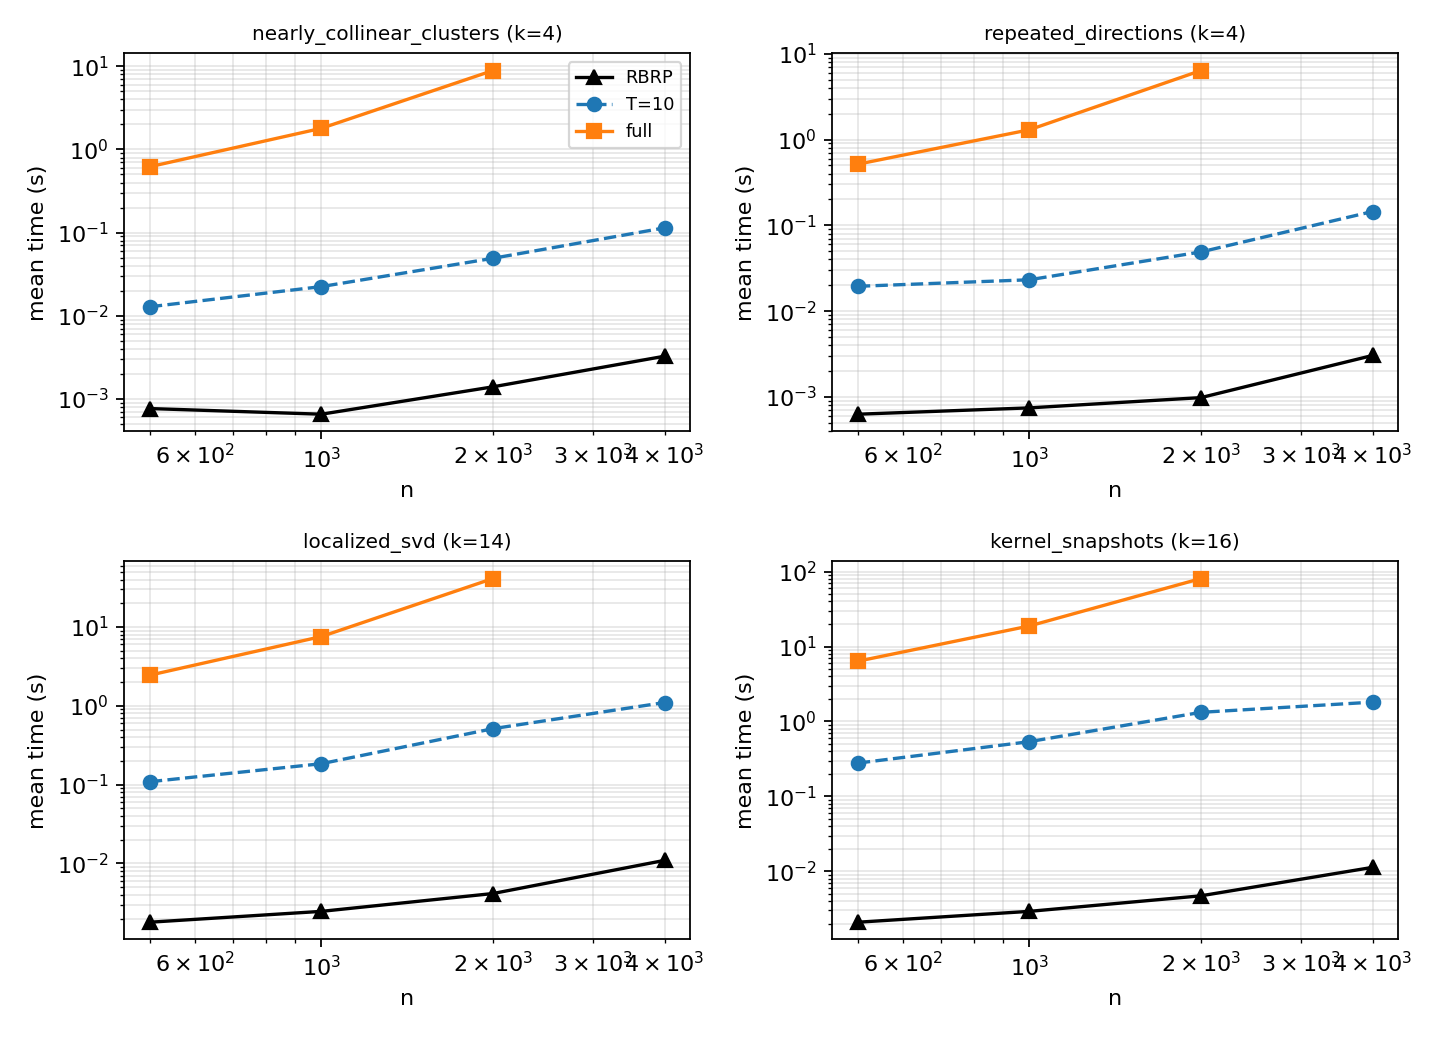
\includegraphics[width=.8\textwidth]{figs/runtime.png}
\caption{Mean wall-clock time versus $n$ (log--log).}\label{fig:runtime}\end{figure}
The refinement is substantially more expensive than RBRP itself: with $T=10$ it takes $17$--$281$ times the RBRP time for $n\le4000$ and $0.01$--$1.8$\,s; the full scan ($n\le2000$) takes $800$--$17000$ times RBRP.
Fitted exponents of time in $n$: RBRP $0.72$--$0.86$, $T=10$ $0.94$--$1.15$ (the number of evaluations does not grow with $n$ while each evaluation is linear in $n$), full scan $1.81$--$2.04$, in agreement with Proposition~\ref{prop:cost}; the exponents rest on three or four values of $n$ and few seeds and should be read as orders of magnitude.

\subsection{Refining a QRCP skeleton}
\begin{table}[t]
\centering\small
\caption{Refining the QRCP skeleton (one deterministic run per row).}\label{tab:qrcp}
\begin{adjustbox}{max width=\linewidth}
\begin{tabular}{lrrrrrr}
\toprule
Matrix & $k$ & $A$ (QRCP) & $T{=}10$: $A/A_{\rm QRCP}$ & $E/E_{\rm QRCP}$ & full: $A/A_{\rm QRCP}$ & $E/E_{\rm QRCP}$ \\
\midrule
Burgers & 8 & 13.44 & 1.000 & 0.999 & 0.789 & 1.014 \\
Burgers & 16 & 12.73 & 0.887 & 1.038 & 0.589 & 1.017 \\
Burgers & 24 & 13.30 & 1.000 & 1.000 & 0.837 & 1.024 \\
Digits & 10 & 18.66 & 0.769 & 1.001 & 0.676 & 1.002 \\
Digits & 20 & 15.90 & 0.907 & 1.048 & -- & -- \\
Digits & 30 & 17.00 & 0.932 & 1.023 & -- & -- \\
\bottomrule
\end{tabular}
\end{adjustbox}
\end{table}

Table~\ref{tab:qrcp}: the refinement also lowers the amplification of a QRCP skeleton (full scan by $16$--$41\%$; $T=10$ by $0$--$23\%$, with essentially no effect on Burgers $k=8,24$). This is a single deterministic run per row and is only indicative.

\subsection{Downstream effect of the amplification}\label{sec:noise}
\begin{table}[t]
\centering\small
\caption{Reconstruction error under perturbations of the skeleton, relative to the RBRP skeleton: median over all configurations and 20 seeds of $\mathrm{err}(\text{method})/\mathrm{err}(\text{RBRP})$, with 95\% bootstrap intervals. Random noise: relative level $\nu$; worst case: relative size $\eta$ (lower bound of Proposition~\ref{prop:pert}). $\rho_A,\rho_F$: median ratios of $\|W\|_2$, $\|W\|_F$. Last row: paired ratio of the pipeline to the guarded volume exchange. For $0.01$ the differences are dominated by those in $E$.}\label{tab:noise}
\begin{adjustbox}{max width=\linewidth}
\begin{tabular}{lrrrrrr}
\toprule
 & $\rho_A$ & $\rho_F$ & \multicolumn{2}{c}{random noise $\nu$} & \multicolumn{2}{c}{worst case $\eta$}\\
\cmidrule(lr){4-5}\cmidrule(lr){6-7}
Method & & & 0.1 & 1 & 0.1 & 1 \\
\midrule
Vol(1) & 0.56 [0.52,0.58] & 0.64 [0.60,0.68] & 0.86 [0.85,0.88] & 0.71 [0.70,0.74] & 0.75 [0.73,0.78] & 0.64 [0.59,0.68] \\
VolGuard & 0.60 [0.57,0.64] & 0.68 [0.66,0.70] & 0.85 [0.84,0.86] & 0.73 [0.71,0.75] & 0.76 [0.73,0.78] & 0.68 [0.64,0.71] \\
Ours-$T$10 & 0.61 [0.57,0.63] & 0.72 [0.69,0.77] & 0.96 [0.94,0.96] & 0.81 [0.79,0.83] & 0.81 [0.79,0.86] & 0.69 [0.65,0.73] \\
Hybrid & 0.56 [0.53,0.59] & 0.67 [0.65,0.69] & 0.86 [0.85,0.89] & 0.73 [0.70,0.75] & 0.73 [0.70,0.76] & 0.63 [0.59,0.66] \\
Hybrid/VolGuard (paired) & -- & -- & 1.000 [1.000,1.004] & 1.000 [1.000,1.000] & 1.000 [0.999,1.000] & 0.964 [0.948,0.974] \\
\bottomrule
\end{tabular}
\end{adjustbox}
\end{table}

\begin{table}[t]
\centering\small
\caption{Crossover noise level $\nu^*=E_0\sqrt n/\|W_0\|_F$ of the RBRP skeletons (median and quartiles over 20 seeds): the random-noise term of the reconstruction error exceeds the approximation error only for $\nu>\nu^*$.}\label{tab:nustar}
\begin{adjustbox}{max width=\linewidth}
\begin{tabular}{lrrr}
\toprule
Matrix & $k$ & median $\nu^*$ & quartiles \\
\midrule
Burgers & 8 & 0.134 & [0.105, 0.163] \\
Burgers & 16 & 0.0379 & [0.0316, 0.0443] \\
Burgers & 24 & 0.00366 & [0.0031, 0.00461] \\
Digits & 10 & 0.472 & [0.451, 0.488] \\
Digits & 20 & 0.252 & [0.248, 0.257] \\
Digits & 30 & 0.135 & [0.131, 0.14] \\
Kernel snapshots & 16 & 0.027 & [0.0209, 0.033] \\
Localized SVD & 14 & 0.0132 & [0.0107, 0.0213] \\
Collinear clusters & 4 & 2.27 & [1.79, 3.04] \\
Repeated directions & 4 & 0.949 & [0.884, 1.1] \\
\bottomrule
\end{tabular}
\end{adjustbox}
\end{table}

\begin{figure}[t]\centering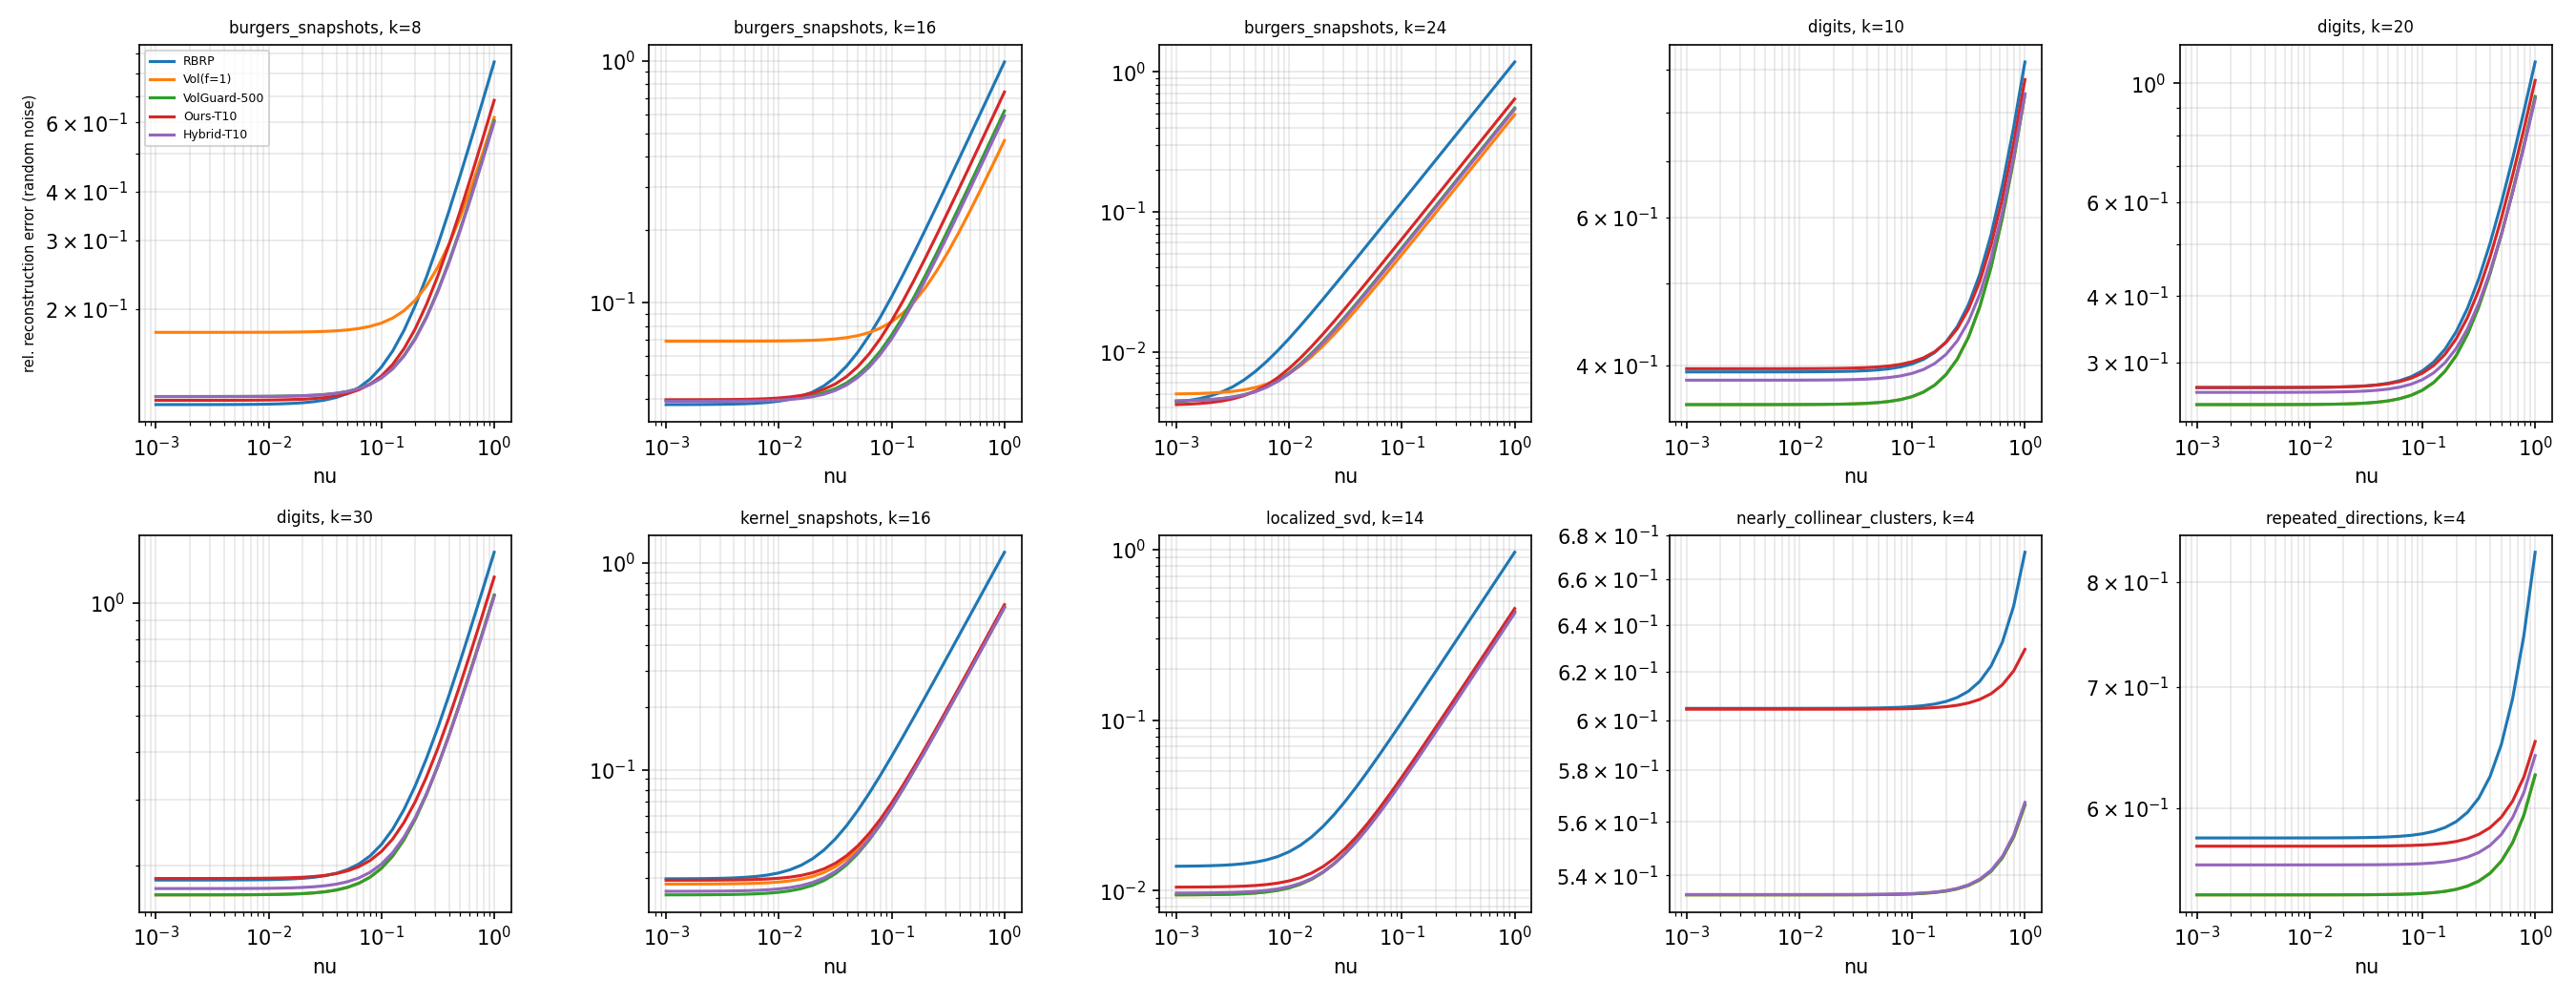
\includegraphics[width=\textwidth]{figs/noise_random.png}
\caption{Expected relative reconstruction error under random noise of relative level $\nu$ (median skeleton per method).}\label{fig:noiserand}\end{figure}
\begin{figure}[t]\centering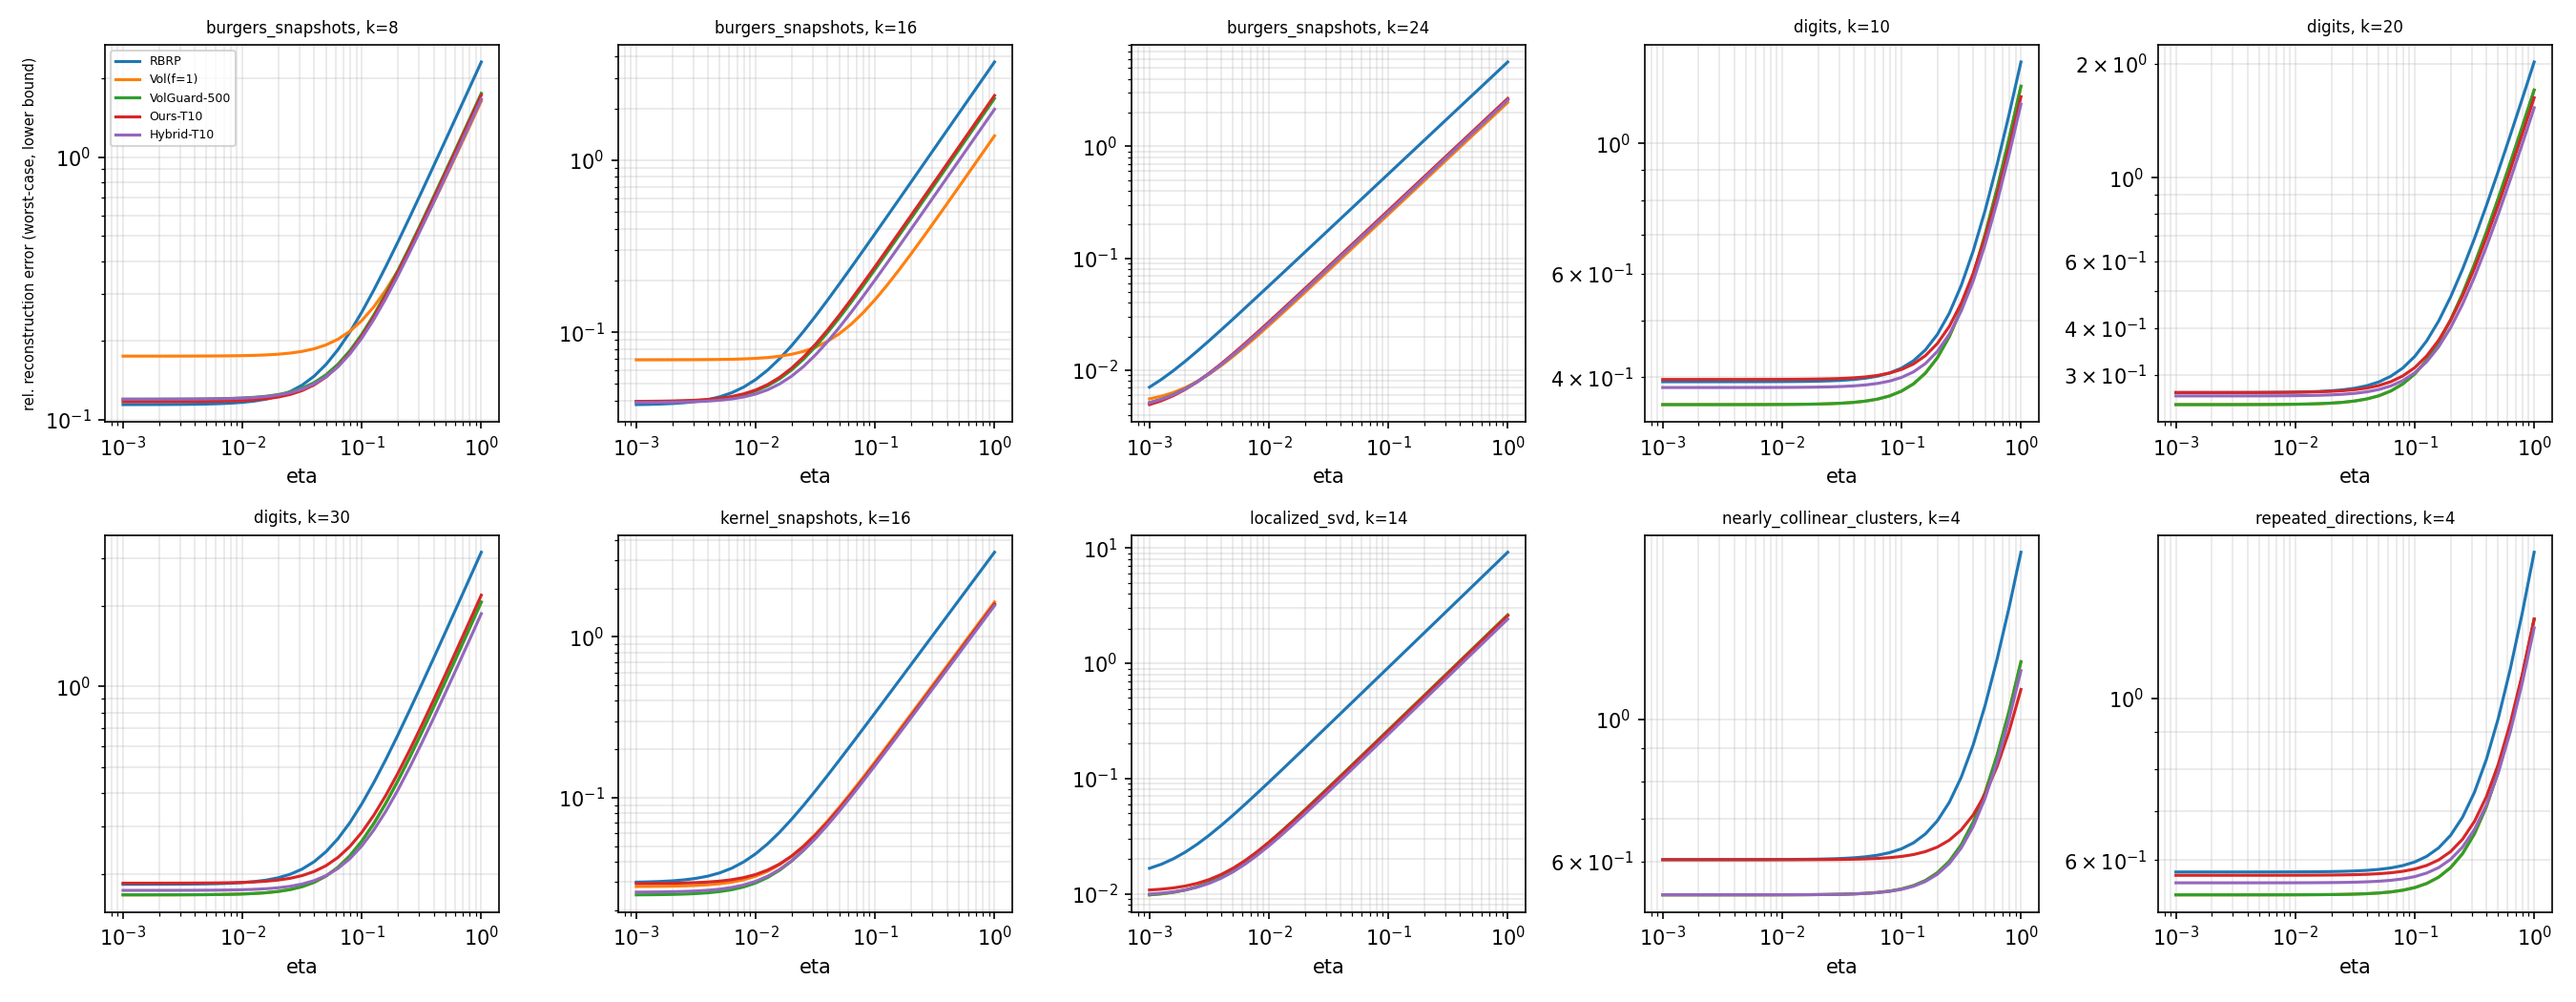
\includegraphics[width=\textwidth]{figs/noise_worst.png}
\caption{Lower bound on the worst-case relative reconstruction error for perturbations of relative size $\eta$.}\label{fig:noiseworst}\end{figure}
We evaluate the reconstruction $\hat X=W(X_S+N)$ with the closed forms of Proposition~\ref{prop:pert}; a Monte-Carlo check with 100 draws agrees with formula (a) to within about $1\%$ in all 20 tested cases.
Over all skeletons, $\log\|W\|_2$ and $\log\|W\|_F$ are strongly correlated (correlation $0.94$) and $\|W\|_2/\|W\|_F$ has median $0.55$.
\begin{itemize}
\item \emph{Lower amplification lowers the error under perturbations (Table~\ref{tab:noise}).} At a large perturbation, the pipeline reduces the median reconstruction error of the RBRP skeleton by $27\%$ for random noise ($\nu=1$; interval of the ratio $0.705$--$0.746$) and by $37\%$ in the worst case ($\eta=1$; $0.595$--$0.660$); the Frobenius norm $\|W\|_F$ falls in $98.5\%$ of the runs (median ratio $0.67$, against $0.56$ for $\|W\|_2$).
\item \emph{The benefit appears only above a matrix-dependent noise level (Table~\ref{tab:nustar}).} The crossover $\nu^*$ ranges from about $0.004$ to $2.3$ (relative to the rms entry of $X$): for localized SVD, kernel snapshots and the Burgers matrix at $k=24$ the benefit is visible at noise of a few percent, for the collinear and repeated-direction matrices only for noise comparable to the signal. For small perturbations the error is dominated by $E$, and the differences in Table~\ref{tab:noise} at $0.01$ are mostly differences in $E$.
\item \emph{The second stage adds little to the perturbed reconstruction.} Paired against the guarded volume exchange, the error ratio of the pipeline is $1.000$ with intervals inside $[0.999,1.008]$ for all random-noise levels and for worst-case perturbations up to $\eta=0.1$; only at $\eta=1$ is it smaller, by $3.6\%$ ($0.948$--$0.974$). So the additional reduction of $\|W\|_2$ obtained by the refinement pays off for the perturbed reconstruction only for large worst-case perturbations. The refinement alone at $T=10$ is worse than the pipeline and the guarded volume exchange under random noise.
\item \emph{Unguarded volume exchange can hurt for small perturbations.} On the Burgers matrix at $k=8,16$ its error stays above that of the RBRP skeleton until $\eta\approx0.03$--$0.1$ because it increases $E$ (Figure~\ref{fig:noiseworst}).
\end{itemize}
These are medians of ratios pooled over configurations; the proxy does not replace an application study (e.g.\ a full DEIM solve).

\subsection{Additional real matrices}\label{sec:real}
\begin{table}[t]
\centering\small
\caption{Additional real matrices (10 RBRP seeds): median amplification $A$ after each method and the share of Vol(1) runs satisfying $E\le1.05E_0$.}\label{tab:real}
\begin{adjustbox}{max width=\linewidth}
\begin{tabular}{lrrrrrrrr}
\toprule
Matrix & $k$ & RBRP & QRCP & Vol(1) & VolGuard & Ours-$T$10 & Hybrid & Vol(1) feasible \\
\midrule
Digits kernel & 8 & 20.9 & 14.2 & 13.0 & 13.0 & 13.2 & 12.7 & 100\% \\
Digits kernel & 16 & 18.2 & 12.3 & 11.9 & 11.9 & 12.0 & 10.9 & 100\% \\
Digits kernel & 32 & 15.4 & 10.6 & 11.2 & 11.2 & 10.7 & 9.6 & 100\% \\
ECG Hankel & 8 & 21.5 & 15.6 & 13.1 & 13.1 & 13.2 & 12.9 & 100\% \\
ECG Hankel & 16 & 26.0 & 17.7 & 14.7 & 14.7 & 14.2 & 13.0 & 100\% \\
ECG Hankel & 32 & 36.9 & 17.4 & 15.4 & 16.0 & 20.9 & 15.0 & 0\% \\
Image patches & 8 & 33.5 & 28.1 & 22.2 & 24.3 & 32.3 & 16.3 & 0\% \\
Image patches & 16 & 33.8 & 28.5 & 15.6 & 16.3 & 22.0 & 12.3 & 40\% \\
Image patches & 32 & 33.9 & 27.9 & 13.2 & 13.0 & 10.3 & 10.2 & 70\% \\
\bottomrule
\end{tabular}
\end{adjustbox}
\end{table}

\begin{table}[t]
\centering\small
\caption{Pipeline versus QRCP (median over seeds of the ratios; QRCP is a single deterministic skeleton) and mean wall-clock times.}\label{tab:realqrcp}
\begin{adjustbox}{max width=\linewidth}
\begin{tabular}{lrrrrrr}
\toprule
Matrix & $k$ & Hybrid $A/A_{\rm QRCP}$ & Hybrid $E/E_{\rm QRCP}$ & Vol(1) time (s) & Ours-$T$10 time (s) & Hybrid time (s) \\
\midrule
Digits kernel & 8 & 0.89 & 1.02 & 0.63 & 2.3 & 2.2 \\
Digits kernel & 16 & 0.89 & 1.01 & 0.63 & 5.7 & 5.5 \\
Digits kernel & 32 & 0.90 & 1.01 & 0.64 & 25.7 & 19.0 \\
ECG Hankel & 8 & 0.83 & 0.90 & 0.09 & 2.2 & 0.9 \\
ECG Hankel & 16 & 0.73 & 0.97 & 0.10 & 7.2 & 3.3 \\
ECG Hankel & 32 & 0.86 & 0.72 & 0.14 & 20.3 & 9.6 \\
Image patches & 8 & 0.58 & 1.16 & 0.04 & 1.1 & 1.7 \\
Image patches & 16 & 0.43 & 1.10 & 0.05 & 5.0 & 4.7 \\
Image patches & 32 & 0.37 & 1.08 & 0.06 & 26.4 & 16.5 \\
\bottomrule
\end{tabular}
\end{adjustbox}
\end{table}

\begin{table}[t]
\centering\small
\caption{Additional real matrices: paired comparison pooled over the nine configurations and ten seeds, with 95\% bootstrap intervals (as in Table~\ref{tab:pooled}).}\label{tab:realpooled}
\begin{adjustbox}{max width=\linewidth}
\begin{tabular}{llrrrrr}
\toprule
x & y & pairs & median $A$ ratio & median $E$ ratio & x dominates (\%) & y dominates (\%) \\
\midrule
Ours-T10 & Vol(f=1) & 90 & 1.031 [0.980, 1.062] & 1.093 [1.061, 1.106] & 7.8 [3.3, 12.2] & 26.7 [20.0, 33.3] \\
Ours-T10 & VolGuard-500 & 90 & 1.030 [0.981, 1.054] & 1.099 [1.075, 1.114] & 5.6 [2.2, 10.0] & 35.6 [26.7, 44.4] \\
Hybrid-T10 & VolGuard-500 & 90 & 0.893 [0.866, 0.922] & 1.029 [1.017, 1.042] & 16.7 [11.1, 23.3] & 0.0 [0.0, 0.0] \\
Hybrid-T10 & Ours-T10 & 90 & 0.896 [0.880, 0.922] & 0.985 [0.964, 0.997] & 48.9 [38.9, 57.8] & 7.8 [3.3, 12.2] \\
Hybrid-T10 & Vol(f=1) & 90 & 0.917 [0.885, 0.943] & 1.015 [1.010, 1.033] & 23.3 [16.7, 30.0] & 0.0 [0.0, 0.0] \\
Ours-T10-noG & Vol(f=1) & 90 & 0.947 [0.924, 0.984] & 1.119 [1.099, 1.126] & 6.7 [2.2, 11.1] & 28.9 [21.1, 36.7] \\
\bottomrule
\end{tabular}
\end{adjustbox}
\end{table}

\begin{figure}[t]\centering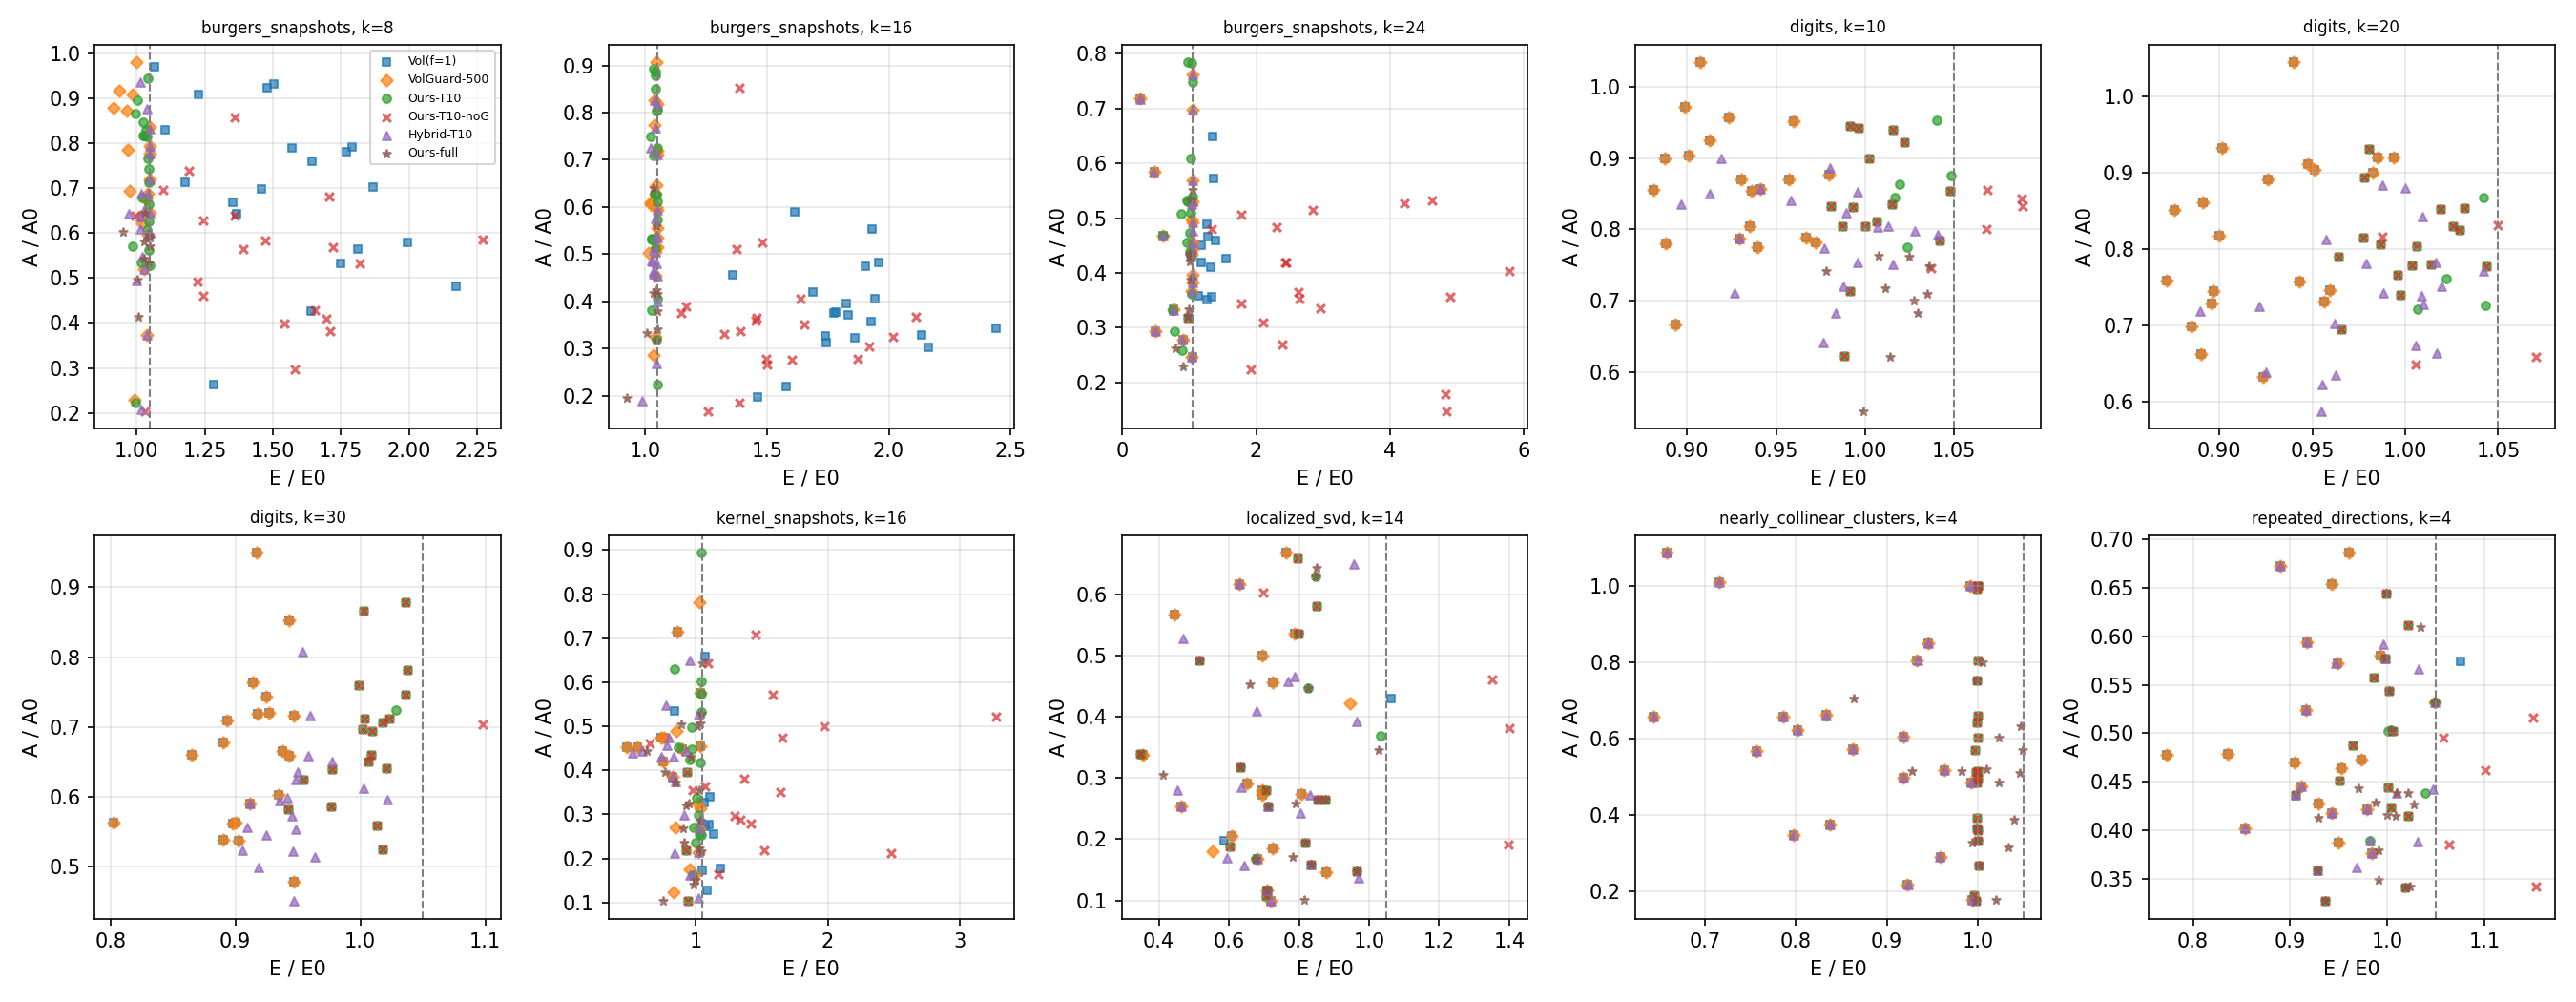
\includegraphics[width=\textwidth]{figs/scatter_real.png}
\caption{Per-run $(E/E_0,A/A_0)$ on the additional real matrices; the dashed line is the budget $1.05$.}\label{fig:scatterreal}\end{figure}
To test whether the findings carry over to public real data we added three matrices, with ranks $k=8,16,32$ and 10 RBRP seeds each:
\emph{image patches}, $3000$ random $12\times12$ gray-scale patches (values in $[0,1]$) from four scikit-image test images, a $3000\times144$ matrix (optimal relative rank-$k$ error $0.10,0.078,0.058$);
\emph{ECG}, the delay-embedding matrix (windows of 128 samples, stride 10, $3588$ rows) of the first $36{,}000$ standardized samples of the ECG record distributed with SciPy ($0.26,0.14,0.045$);
\emph{digits kernel}, the $1000\times1000$ Gaussian kernel matrix (bandwidth equal to the median pairwise distance) of 1000 randomly chosen handwritten digits ($0.045,0.023,0.010$).
The protocol is that of the previous experiments; no full scan was run.
Tables~\ref{tab:real}--\ref{tab:realpooled} and Figure~\ref{fig:scatterreal} show:
\begin{itemize}
\item Unguarded volume exchange violates the budget in 29 of 90 runs ($32\%$, Wilson interval $24$--$42\%$; maximum $E=1.39E_0$), in all runs on image patches at $k=8$ and on ECG at $k=32$; together with Section~\ref{sec:exp} this is 93 of 290 runs ($32\%$). The guarded methods satisfy the budget in all runs.
\item The refinement alone at $T=10$ is again not better than the guarded volume exchange (median $A$ ratio $1.030$, interval $0.981$--$1.054$; error ratio $1.099$, $1.075$--$1.114$; the guarded volume exchange dominates in $35.6\%$ of the pairs, the refinement in $5.6\%$) and stalls at larger ranks: on ECG at $k=32$ its median amplification is $20.9$ against $16.0$ for VolGuard and $15.0$ for the pipeline.
\item The pipeline gains more over the guarded volume exchange than on the earlier matrices: median $A$ ratio $0.893$ ($0.866$--$0.922$), smaller in $88\%$ of the pairs at an error ratio of $1.029$ ($1.017$--$1.042$); against the refinement alone $0.896$ ($0.880$--$0.922$), dominating in $48.9\%$ of the pairs. The gain is concentrated on image patches (ratios $0.74$--$0.76$ at all three ranks) and on the digits kernel at $k=32$ ($0.86$); on ECG at $k=8$ the two coincide in $80\%$ of the runs. The pooled median of $\rho_A$ is $0.49$ ($0.46$--$0.56$).
\item Compared with QRCP, which is not a competitive baseline here (its amplification is $28$ on image patches), the pipeline has a smaller amplification in $97\%$ of the runs (median $A/A_{\mathrm{QRCP}}$ between $0.37$ and $0.90$); its error is between $0.72$ and $1.16$ times that of QRCP, $8$--$16\%$ higher on image patches, and in $44\%$ of the runs it is better in both quantities.
\item The refinement is expensive on these larger matrices (up to $26$\,s for $T=10$ at $n=3000$, $k=32$; pipeline up to $19$\,s), whereas Vol(1) takes at most $0.64$\,s.
\end{itemize}

\section{Discussion}\label{sec:disc}
We studied post-processing of RBRP skeletons under an explicit error budget.
The main findings are that the amplification of RBRP skeletons is large and not controlled by the approximation error; that post-processing should respect an error budget, because unguarded volume exchange can inflate the error considerably on snapshot-type matrices; and that a two-stage pipeline gives a modest additional reduction of the amplification over guarded volume exchange (median ratio $0.963$, interval $0.937$--$0.976$; $0.893$, $0.866$--$0.922$ on three additional real matrices) at similar cost, while a full scan gives a larger reduction at a much higher cost.

\paragraph{Limitations.}
(i) The contribution is relative to RBRP: QRCP is faster than the refinement; on the matrices of Section~\ref{sec:exp} it gives an amplification comparable to that after the budgeted refinement, whereas on the three additional real matrices the pipeline has a $10$--$63\%$ smaller amplification than QRCP, at an error up to $16\%$ higher; reasons to start from RBRP (scalability, randomization) were not tested here.
(ii) We prove termination and local optimality, not an accuracy guarantee, and not a bound comparable to strong RRQR.
(iii) The refinement costs one to two orders of magnitude more than RBRP; cheaper evaluation (e.g.\ incremental updates) was not explored.
(iv) The volume baseline uses the SVD basis, is not the original strong RRQR implementation, and VolGuard is our own variant.
(v) The downstream evidence is a perturbation proxy: the benefit for random noise is similar to that of guarded volume exchange and appears only above a matrix-dependent noise level; (vi) Data are synthetic matrices, one snapshot matrix generated by us (whose floating-point generation makes the results reproducible only to a few percent across machines), and four small public real matrices (digits, image patches, an ECG delay matrix, a digits kernel matrix; at most $3600\times1000$) whose construction (patch size, bandwidth, window length) we chose; the full scan has only 10 seeds on Burgers and digits $k{=}10$ and none on digits $k{=}20,30$; the budget $T=10$ and $\varepsilon=0.05$ are working points.

\paragraph{Future work.}
Combining the pipeline with other initializations, an incremental implementation of the exact evaluations, and a probabilistic analysis for incoherent low-rank-plus-noise matrices.

\begin{thebibliography}{99}
\bibitem{cheng2005} H.~Cheng, Z.~Gimbutas, P.-G.~Martinsson, V.~Rokhlin, On the compression of low rank matrices, SIAM J. Sci. Comput. 26 (2005) 1389--1404.
\bibitem{dong2025rbrp} Y.~Dong, C.~Chen, P.-G.~Martinsson, K.~Pearce, Robust blockwise random pivoting: fast and accurate adaptive interpolative decomposition, SIAM J. Matrix Anal. Appl. 46 (2025) 1791--1815.
\bibitem{dongmartinsson2023} Y.~Dong, P.-G.~Martinsson, Simpler is better: a comparative study of randomized pivoting algorithms for CUR and interpolative decompositions, Adv. Comput. Math. 49 (2023).
\bibitem{hqrrp2017} P.-G.~Martinsson, G.~Quintana-Ort\'i, N.~Heavner, R.~van de Geijn, Householder QR factorization with randomization for column pivoting (HQRRP), SIAM J. Sci. Comput. 39 (2017) C96--C115.
\bibitem{voronin2017} S.~Voronin, P.-G.~Martinsson, Efficient algorithms for CUR and interpolative matrix decompositions, Adv. Comput. Math. 43 (2017) 495--516.
\bibitem{gu1996} M.~Gu, S.~C.~Eisenstat, Efficient algorithms for computing a strong rank-revealing QR factorization, SIAM J. Sci. Comput. 17 (1996) 848--869.
\bibitem{goreinov2010} S.~A.~Goreinov, I.~V.~Oseledets, D.~V.~Savostyanov, E.~E.~Tyrtyshnikov, N.~L.~Zamarashkin, How to find a good submatrix, in Matrix Methods: Theory, Algorithms and Applications, World Scientific, 2010, pp.~247--256.
\bibitem{mikhalev2018} A.~Mikhalev, I.~V.~Oseledets, Rectangular maximum-volume submatrices and their applications, Linear Algebra Appl. 538 (2018) 187--211.
\bibitem{osinsky2026} A.~Osinsky, I.~Kozyrev, Subset selection for matrices by column exchange, arXiv:2604.14418, 2026.
\bibitem{kozyrev2026} I.~Kozyrev, A.~Osinsky, Subset selection for matrices in spectral norm, arXiv:2507.20435, 2025.
\bibitem{cortinovisying2025} A.~Cortinovis, L.~Ying, A sublinear-time randomized algorithm for column and row subset selection based on strong rank-revealing QR factorizations, SIAM J. Matrix Anal. Appl. 46 (2025) 22--44.
\bibitem{grigori2025} L.~Grigori, Z.~Xue, Randomized strong rank-revealing QR for column subset selection and low-rank matrix approximation, arXiv:2503.18496, 2025.
\bibitem{chaturantabut2010} S.~Chaturantabut, D.~C.~Sorensen, Nonlinear model reduction via discrete empirical interpolation, SIAM J. Sci. Comput. 32 (2010) 2737--2764.
\bibitem{drmac2016} Z.~Drma\v{c}, S.~Gugercin, A new selection operator for the discrete empirical interpolation method---improved a priori error bound and extensions, SIAM J. Sci. Comput. 38 (2016) A631--A648.
\bibitem{sorensen2016} D.~C.~Sorensen, M.~Embree, A DEIM induced CUR factorization, SIAM J. Sci. Comput. 38 (2016) A1454--A1482.
\bibitem{peherstorfer2020} B.~Peherstorfer, Z.~Drma\v{c}, S.~Gugercin, Stability of discrete empirical interpolation and gappy proper orthogonal decomposition with randomized and deterministic sampling points, SIAM J. Sci. Comput. 42 (2020). % VERIFY pages
\bibitem{murray2023} R.~Murray et al., Randomized numerical linear algebra: a perspective on the field with an eye to software, arXiv:2302.11474, 2023.
\bibitem{madan2019} V.~Madan, M.~Singh, U.~Tantipongpipat, W.~Xie, Combinatorial algorithms for optimal design, Proc. COLT, PMLR 99 (2019) 2210--2258.
\bibitem{chen2025rpchol} Y.~Chen, E.~N.~Epperly, J.~A.~Tropp, R.~J.~Webber, Randomly pivoted Cholesky: practical approximation of a kernel matrix with few entry evaluations, Comm. Pure Appl. Math. (2025), arXiv:2207.06503.
\bibitem{epperly2025accel} E.~N.~Epperly, J.~A.~Tropp, R.~J.~Webber, Embrace rejection: kernel matrix approximation by accelerated randomly pivoted Cholesky, SIAM J. Matrix Anal. Appl. 46 (2025) 2527--2557.
\bibitem{pearce2025lupp} K.~Pearce, C.~Chen, Y.~Dong, P.-G.~Martinsson, Adaptive parallelizable algorithms for interpolative decompositions via partially pivoted LU, Numer. Linear Algebra Appl. 32 (2025) e70002.
\bibitem{cortinovis2026arp} A.~Cortinovis, D.~Kressner, Adaptive randomized pivoting for column subset selection, DEIM, and low-rank approximation, SIAM J. Matrix Anal. Appl. 47 (2026), arXiv:2412.13992.
\bibitem{epperly2026arp} E.~N.~Epperly, Adaptive randomized pivoting and volume sampling, SIAM J. Matrix Anal. Appl. 47 (2026) 1785--1798.
\bibitem{pearcemartinsson2026} K.~J.~Pearce, P.-G.~Martinsson, Randomized algorithms for low-rank matrix and tensor decompositions, in Numerical Analysis and Scientific Computing: an Anthology, Springer, 2026, pp.~197--252.
\bibitem{parknak2025} T.~Park, Y.~Nakatsukasa, Accuracy and stability of CUR decompositions with oversampling, SIAM J. Matrix Anal. Appl. 46 (2025) 780--810.
\bibitem{parknak2025param} T.~Park, Y.~Nakatsukasa, Low-rank approximation of parameter-dependent matrices via CUR decomposition, SIAM J. Sci. Comput. 47 (2025) A1858--A1887.
\bibitem{cutforth2026} M.~Cutforth, T.~Fan, T.~Zahtila, A.~Doostan, E.~Darve, Bi-fidelity interpolative decomposition for multimodal data, Comput. Methods Appl. Mech. Engrg. 451 (2026) 118706.
\bibitem{patel2025} V.~Patel et al., Scientific applications leveraging randomized linear algebra, arXiv:2506.16457, 2025.
\bibitem{lazzarino2026} L.~Lazzarino, K.~J.~Pearce, N.~Pritchard, Blind error estimation for CUR approximation, arXiv:2609.23810, 2026.
\bibitem{damle2026} A.~Damle, Computing strong rank-revealing factorizations for matrices with orthonormal rows, arXiv:2607.13532, 2026.
\bibitem{osinsky2024} A.~I.~Osinsky, Volume-based subset selection, Numer. Linear Algebra Appl. 31 (2024) e2525.
\bibitem{kozyrev2026vs} I.~Kozyrev, A.~Osinsky, Subset selection for matrices by volume sampling, arXiv:2610.08576, 2026.
\bibitem{avron2013} H.~Avron, C.~Boutsidis, Faster subset selection for matrices and applications, SIAM J. Matrix Anal. Appl. 34 (2013) 1464--1499.
\bibitem{drineas2008} P.~Drineas, M.~W.~Mahoney, S.~Muthukrishnan, Relative-error CUR matrix decompositions, SIAM J. Matrix Anal. Appl. 30 (2008) 844--881.
\bibitem{chiudemanet2013} J.~Chiu, L.~Demanet, Sublinear randomized algorithms for skeleton decompositions, SIAM J. Matrix Anal. Appl. 34 (2013) 1361--1383.
\bibitem{fedorov1972} V.~V.~Fedorov, Theory of Optimal Experiments, Academic Press, 1972.
\end{thebibliography}
\end{document}
